% compress:
% gs -sDEVICE=pdfwrite -dCompatibilityLevel=1.4 -dNOPAUSE -dQUIET -dBATCH      -sOutputFile=CompressedSwarmControlJournal.pdf SwarmControlJournal.pdf
%%%%%%%%% IJRR SETTINGS
%  from https://us.sagepub.com/en-us/nam/manuscript-submission-guidelines#PreparingYourManuscript
%\documentclass[Afour,sageh,times]{sagej} % sage_latex_guidelines.tex V1.01, 11 June 2015
\documentclass[conference]{IEEEtran}
\IEEEoverridecommandlockouts% This command is only needed if 
                                                          % you want to use the \thanks command
%\overrideIEEEmargins                                      % Needed to meet printer requirements.
\usepackage{times}


\makeatletter 
\let\NAT@parse\undefined
\makeatother

% numbers option provides compact numerical references in the text. 
%\usepackage[numbers]{natbib}
\usepackage{multicol}


\usepackage{bbm}
\usepackage{calc}
\usepackage{url}
\usepackage{transparent}
\usepackage[hidelinks]{hyperref}
\hypersetup{
  colorlinks =false,
  urlcolor = black,
  linkcolor = black,
  citecolor = black
}
\usepackage{graphicx}
\usepackage[cmex10]{amsmath}
\usepackage{bm}
\usepackage{amssymb}
\usepackage{rotating}

\usepackage{chngcntr}
\counterwithin{paragraph}{subsection} % makes paragraph depend on subsection

\usepackage{nicefrac}
\usepackage{cite}
\usepackage[caption=false,font=footnotesize]{subfig}
\usepackage[usenames, dvipsnames]{color}
\usepackage{colortbl}
\usepackage{overpic}
\graphicspath{{./}}
\usepackage{breqn} %for breaking equations automatically
\usepackage[ruled]{algorithm}
\usepackage{algpseudocode}
\usepackage{multirow}
\usepackage{todonotes}
\usepackage{authblk}
\usepackage{flushend}

%\newcommand{\todo}[1]{\vspace{5 mm}\par \noindent \framebox{\begin{minipage}[c]{0.98 \columnwidth} \ttfamily\flushleft \textcolor{red}{#1}\end{minipage}}\vspace{5 mm}\par}
% uncomment this to hide all red todos
%\renewcommand{\todo}{}

%% ABBREVIATIONS
\newcommand{\qstart}{q_{\text{start}}}



%% MACROS


\providecommand{\abs}[1]{\left\lvert#1\right\rvert}
\providecommand{\norm}[1]{\left\lVert#1\right\rVert}
\providecommand{\normn}[2]{\left\lVert#1\right\rVert_#2}
\providecommand{\dualnorm}[1]{\norm{#1}_\ast}
\providecommand{\dualnormn}[2]{\norm{#1}_{#2\ast}}
\providecommand{\set}[1]{\lbrace\,#1\,\rbrace}
\providecommand{\cset}[2]{\lbrace\,{#1}\nobreak\mid\nobreak{#2}\,\rbrace}
\providecommand{\lscal}{<}
\providecommand{\gscal}{>}
\providecommand{\lvect}{\prec}
\providecommand{\gvect}{\succ}
\providecommand{\leqscal}{\leq}
\providecommand{\geqscal}{\geq}
\providecommand{\leqvect}{\preceq}
\providecommand{\geqvect}{\succeq}
\providecommand{\onevect}{\mathbf{1}}
\providecommand{\zerovect}{\mathbf{0}}
\providecommand{\field}[1]{\mathbb{#1}}
\providecommand{\C}{\field{C}}
\providecommand{\R}{\field{R}}
\newcommand{\Cspace}{\mathcal{Q}}
\newcommand{\Uspace}{\mathcal{U}}
\providecommand{\Fspace}{\Cspace_\text{free}}
\providecommand{\Hcal}{$\mathcal{H}$}
\providecommand{\Vcal}{$\mathcal{V}$}
\DeclareMathOperator{\conv}{conv}
\DeclareMathOperator{\cone}{cone}
\DeclareMathOperator{\homog}{homog}
\DeclareMathOperator{\domain}{dom}
\DeclareMathOperator{\range}{range}
\DeclareMathOperator{\sign}{sgn}
\providecommand{\polar}{\triangle}
\providecommand{\ainner}{\underline{a}}
\providecommand{\aouter}{\overline{a}}
\providecommand{\binner}{\underline{b}}
\providecommand{\bouter}{\overline{b}}
\newcommand{\D}{\nobreakdash-\textsc{d}}
\providecommand{\Fspace}{\Cspace_\text{free}}
\providecommand{\free}{\text{\{}\mathsf{free}\text{\}}}
\providecommand{\iff}{\Leftrightarrow}
\providecommand{\subinner}[1]{#1_{\text{inner}}}
\providecommand{\subouter}[1]{#1_{\text{outer}}}
\providecommand{\Ppoly}{\mathcal{X}}
\providecommand{\Pproj}{\mathcal{Y}}
\providecommand{\Pinner}{\subinner{\Pproj}}
\providecommand{\Pouter}{\subouter{\Pproj}}
\DeclareMathOperator{\argmax}{arg\,max}
\providecommand{\Aineq}{B}
\providecommand{\Aeq}{A}
\providecommand{\bineq}{u}
\providecommand{\beq}{t}
\DeclareMathOperator{\area}{area}
\newcommand{\contact}[1]{\Cspace_{#1}}
\newcommand{\feasible}[1]{\Fspace_{#1}}
\newcommand{\dd}{\; \mathrm{d}}
\newcommand{\figwid}{0.22\columnwidth}
\newcommand{\TRUE}{\textbf{true}}
\newcommand{\FALSE}{\textbf{false}}
\DeclareMathOperator{\atan2}{atan2}
\allowdisplaybreaks

\newtheorem{theorem}{Theorem}
\newtheorem{definition}[theorem]{Definition}
\newtheorem{lemma}[theorem]{Lemma}


%useful for highlighting sections that need work
%\newcommand{\todo}[1]{\textcolor{red}{\footnotesize \textsf{#1}}}


%\setcounter{secnumdepth}{3}
%\runninghead{Shahrokhi \textit{et~al.}}
%\hyphenation{micro-robot nano-robot nano-robotics micro-robotics micro-robots nano-robots micro-manip-ulators}
%%%%%%%%%%%% For debugging purposes, I like to display the TOC
%    \tableofcontents
%    \setcounter{tocdepth}{3}
%    \newpage
%%%% END TOC %%%%%%%%%%%%%%%%%%%%%%%%%%%%%%%%%%%%%%%
 

\title{\LARGE \bf Steering a Swarm of Particles\\ Using Global Inputs and Swarm Statistics}

\author{Shiva Shahrokhi, Lillian Lin, Chris Ertel, Mable Wan,  Aaron T. Becker% end author block 
\thanks{This work was supported by the National Science Foundation under Grant No.\ \href{http://nsf.gov/awardsearch/showAward?AWD_ID=1553063}{[IIS-1553063]}.}% <-this % stops a space
\thanks{Authors are with the Department of Electrical and Computer Engineering,  University of Houston, Houston, TX 77204 USA        {\tt\small  \{sshahrokhi2, atbecker\}@uh.edu}}
}

\begin{document}

\maketitle
\thispagestyle{empty}
\pagestyle{empty}
\begin{abstract}
Microrobotics has the potential to revolutionize many applications including targeted material delivery, assembly, and surgery.  The same properties that promise breakthrough solutions---small size and large populations---present unique challenges for controlling motion. 
Robotic manipulation usually assumes intelligent agents, not particle systems manipulated by a global signal.
To identify the key parameters for particle manipulation, we used a collection of online games where players steer swarms of up to 500 particles to complete manipulation challenges. We recorded statistics from over ten thousand players. 
Inspired by techniques where human operators performed well, we investigate controllers that use only the mean and variance of the swarm. We prove the mean position is controllable and provide conditions under which variance is controllable.  We next derive automatic controllers for these and a hysteresis-based switching control to regulate the first two moments of the particle distribution. 
Finally, we employ these controllers as primitives for an object manipulation task and implement all controllers on 100 kilobots controlled by the direction of a global light source.
\end{abstract}

\begin{IEEEkeywords}
Multi-robot systems, Robot motion 
\end{IEEEkeywords}

%  TRO       Manipulation Planning, 	Underactuated Robots,   human-swarm interaction,   swarm
%  maybe TRO	Manipulation and Compliant Assembly, 	Path Planning for Multiple Mobile Robot Systems

%Previously presented*  
% [1] A. T. Becker, C. Ertel, and J. McLurkin, �Crowdsourcing swarm manipulation experiments: A massive online user study with large swarms of simple robots,� in IEEE International Conference on Robotics and Automation (ICRA), 2014, pp. 2825�2830.
% [2] S. Shahrokhi and A. T. Becker, �Stochastic swarm control with global inputs,� in IEEE/RSJ International Conference on  Intelligent Robots and Systems (IROS), Sep. 2015, pp. 421�427.


\section{Introduction}\label{sec:Intro}
%This project studies system models and user interfaces for five multi-robot manipulation tasks with large populations of micro- and nanorobots.  We test several system models with different limitations on controllability and observability of the motion controller, and evaluate several different user interfaces.  We conduct user experiments to understand the impact of these limitations and design choices. 


%Micro- and nanorobotics have the potential to revolutionize many applications including targeted material delivery, assembly, and surgery.  The same properties that promise breakthrough solutions---small size and large populations---present unique challenges to generating controlled motion.  
Large populations of micro- and nanorobots are being produced in laboratories around the world, with diverse potential applications in drug delivery and construction, see \cite{Peyer2013,Shirai2005,Chiang2011}. These activities require robots that behave intelligently.
Limited computation and communication rules out autonomous operation or direct control over individual units; instead we must rely on global control signals broadcast to the entire robot population.  Additionally, many promising applications will require direct human control, but user interfaces to thousands---or millions---of robots is a daunting human-swarm interaction (HSI) challenge. 

Our previous work with over a hundred hardware robots and thousands of simulated robots~\cite{Becker2013b} demonstrated that direct human control of large swarms is possible. 
Unfortunately, the logistical challenges of repeated experiments with over one hundred robots prevented large-scale tests. 
There is currently no comprehensive understanding of user interfaces for controlling multi-robot systems with massive populations.  
This paper presents a tool for investigating HSI methods through statistically significant numbers of experiments.  

\begin{figure}
\renewcommand{\figwid}{0.32\columnwidth}
\subfloat[][Vary Number]{\label{fig:VaryNum}
\begin{overpic}[width =\figwid]{VaryNum.pdf}\end{overpic}}
%
\subfloat[][Vary Visual Feedback]{\label{fig:VaryVis}
%\begin{overpic}[width =\figwid]{VaryVisFS.pdf}\end{overpic}
\begin{overpic}[width =\figwid]{VaryVisCH.pdf}\end{overpic}}
%
\subfloat[][Vary Noise]{\label{fig:VaryNoise}
\begin{overpic}[width =\figwid]{VaryNoise.pdf}\end{overpic}}\\
%
\subfloat[][Control Position]{\label{fig:ControlPos}
\begin{overpic}[width =\figwid]{ControlPos.pdf}\end{overpic}}
%
\subfloat[][Vary Control: Assembly]{\label{fig:VaryControl}
\begin{overpic}[width =\figwid]{VaryControl.pdf}\end{overpic}}
%
\subfloat[][Vary Control: Foraging]{\label{fig:Forage}
\begin{overpic}[width =\figwid]{VaryForage.pdf}\end{overpic}}
%
\caption{\label{fig:5experiments}
Screenshots from our online experiments controlling multi-robot systems with limited, global control.
\textbf{(a)} Varying the number of robots from 1-500
\textbf{(b)} Comparing 4 levels of visual feedback 
\textbf{(c)} Varying noise from 0 to 200\% of control authority
\textbf{(d)} Controlling the position of 1 to 10 robots
\textbf{(e)} Comparing 3 control architectures to assemble
\textbf{(f)} Comparing 3 control architectures to forage.
\vspace{-2em}
}
\end{figure}

Our goal was to test several scenarios involving large-scale human-swarm interaction (HSI), and to do so with a statistically-significant sample size. Towards this end, we created \href{http://www.swarmcontrol.net/show_results}{SwarmControl.net}, an open-source, online testing platform suitable for inexpensive deployment and data collection on a scale not yet seen in swarm robotics research. Screenshots from this platform are shown in Fig.~\ref{fig:5experiments}.  \href{https://github.com/crertel/swarmmanipulate.git}{All code} \href{http://www.swarmcontrol.net/show_results}{and experimental results} are posted online, \cite{Chris-Ertel2013}. \todo{TODO: Chris, is 2016 code ready to upload? link to 2016 code}

Our experiments show that numerous simple robots responding to global control inputs are directly controllable by a human operator without special training, that the visual feedback of the swarm state should be simple to increase task performance, and that humans perform swarm-object manipulation faster using attractive control schemes than repulsive control schemes.

%Inspired by our online experiments, because it is not always possible to gather pose information on each robot for feedback control and
%It is not always practical to gather pose information on individual robots for feedback control; the robots might be difficult or impossible to sense individually due to their size and location. However, it is often possible to sense global properties of the group, such as mean position and density.
Often robots are difficult or impossible to sense individually due to their size and location. 
For example, microrobots are smaller than the minimum resolution of a clinical MRI-scanner, see \cite{martel2014computer}, however it is often possible to sense global properties of the group, such as mean position and variance. 
To make progress in automatic control with global inputs, this paper presents swarm manipulation controllers, inspired by our online experiments, that require only mean and variance measurements of the robot's positions.  
These controllers are used as primitives to perform the object manipulation task illustrated in Fig.~\ref{fig:bigPictureMeanAndVarianceForSwarm}.

\begin{figure}
\centering
\begin{overpic}[width=0.5\columnwidth]{CompleteMazeDescription.pdf}\end{overpic}
\begin{overpic}[width=0.438\columnwidth]{MainExpFig.pdf}\end{overpic}
%\todo{I like the 'target' symbol, but it is not self-documenting.  We need a legend explaining the min and max variance ellipses, the goal region, the variance, the mean, the object COM, and the target mean position.  I think these are easiest to make in powerpoint.
%Please use the same color and line style for the variance min and max as you use in Figure 4.
%}
%{blockpushingImageWithMeanAndVarianceOverlay.png}
\caption{\label{fig:bigPictureMeanAndVarianceForSwarm} A swarm of robots, all controlled by a uniform force field, can be effectively controlled by a hybrid controller that knows only the first and second moments of the robot distribution.  Here a swarm of simple robots (blue discs) pushes a green hexagon toward the goal. Simulation at left, screen capture form hardware experiment at right. See multimedia extension.}
\end{figure}
 %function and implementation function

 Our paper is organized as follows.  After a discussion of related work in \S \ref{sec:RelatedWork},  we describe our experimental methods for an online human-user experiment in \S \ref{sec:expMethods}. We report the results of our online experiments in \S \ref{sec:expResults}. Inspired by these results, we prove that the mean and variance of a robot swarm are controllable in \S \ref{sec:theory}, and present automatic controllers in \S \ref{sec:simulation}. We use these controllers as primitives and present a framework for manipulating an object through a maze in \S \ref{sec:exp}. 
 We conclude with implementations of these controllers in on hardware robots and use them to complete an object manipulation task with 100+ kilobots in \S \ref{sec:realExperiment}.
 
 This paper is the synthesis of two preliminary conference papers,  \cite{swarmcontrol2013}, covered first few months of SwarmControl.net experiments, and \cite{ShahrokhiIROS2015}, presented simulations of object manipulation.  This paper presents the final results from SwarmControl.net.  All hardware validation experiments are new.



%%%%%%%%%%%%%%%%%%%%%%%%%%%%%%%%%%%%%%%%%%%%%%%%%%%%%%%%%%%
\section{Related Work}\label{sec:RelatedWork}
%%%%%%%%%%%%%%%%%%%%%%%%%%%%%%%%%%%%%%%%%%%%%%%%%%%%%%%%%%%


%Unlike \emph{caging} manipulation, where robots form a rigid arrangement around an object~\cite{Sudsang2002,Fink2007}, our swarm of robots is unable to grasp the blocks they push, and so our manipulation strategies are similar to \emph{nonprehensile manipulation} techniques, e.g.~\cite{Lynch1999}, where forces must be applied along the center of mass of the moveable object. 


Robotic manipulation by pushing has a long and successful history\cite{Lynch1999,Lynch1996,Akella2000,Bernheisel2006}.  Key developments introduced the notion of stable pushes and a friction cone.  A \emph{stable push} is a pushing operation by a robot with a flat-plate pushing element in which the object does not change orientation relative to the pushing robot\cite{Lynch1999}.  The \emph{friction cone} is the set of vector directions a robot in contact with an object can push that object with a stable push.
Stable pushes can be used as primitives in an rapidly-expanding random tree to form motion plans.
A key difference is that our robots are compliant and tend to flow around the object, making this similar to fluidic trapping~\cite{Armani2006,Becker2009}.  
%\subsection{Block-pushing and Compliant Manipulation}

While ferrous particles tend to clump in a magnetic field, the magnetotactic bacteria of~\cite{martel2015magnetotactic,ou2012motion} are directed by the orientation of the magnetic field and do not suffer from magnetic aggregation.

Controlling the \emph{shape}, or relative positions, of a swarm of robots is a key ability for a myriad of applications.  Correspondingly, it has been studied from a control-theoretic perspective in  both centralized, e.g. virtual leaders in \cite{egerstedt2001formation}, and decentralized approaches, e.g. decentralized control-Lyapunov function controllers in~\cite{hsieh2008decentralized}. Most approaches assume a level of intelligence and autonomy in the individual robots that exceeds the capabilities of current micro- and nano-robots~\cite{martel2015magnetotactic,Xiaohui2015magnetiteMicroswimmers}.
Instead, this chapter focuses on centralized techniques that apply the same control input to each member of the swarm, as in~\cite{Becker2013b}.



%%%%%%%%%%%%%%%%%%%%%%%%%%%%%%%%%%%%%%%%%%%%%%%%%%%%%%%%%%%
\section{Online experiment}
\label{sec:expMethods}
%%%%%%%%%%%%%%%%%%%%%%%%%%%%%%%%%%%%%%%%%%%%%%%%%%%%%%%%%%%

% Experimental Methods
%%  Platform  
%%  Human Subjects
%%% recruited through social media
%%% IRB form  Protocol Number: 14-012E Protocol Title: Massive Manipulation: A n online user study on controlling large swarms of simple robot sApproval Date: 7/26/2013Expiration Date: 7/26/2014
%%% Costs  for experiment:  ??
%%% Instrumenting:
%%%% Google analytics, airbrake, etc.

%% wherein we describe our framework
\begin{figure}
%\centering
\renewcommand{\figwid}{0.3\columnwidth}
\begin{overpic}[width =\figwid]{VaryNum.pdf}	\put(10,80){\textbf{a} }\end{overpic}~
\begin{overpic}[width =\figwid]{VaryVisMV.pdf}	\put(10,80){\textbf{b} }\end{overpic}~
\begin{overpic}[width =\figwid]{VaryNoise.pdf}	\put(10,80){\textbf{c} }\end{overpic}
%\\
%\begin{overpic}[width =\figwid]{ControlPos.pdf}	\put(10,80){\textbf{d} }\end{overpic}~
%\begin{overpic}[width =\figwid]{VaryControl.pdf}	\put(10,80){\textbf{e} }\end{overpic}~
%\begin{overpic}[width =\figwid]{VaryForage.pdf}	\put(10,80){\textbf{f} }\end{overpic}
\caption{\label{fig:5experiments}
Screenshots from our online experiments controlling multi-particle systems with limited, global control.
\textbf{(a)} Varying the number of particles from 1-500
\textbf{(b)} Comparing 4 levels of visual feedback 
\textbf{(c)} Varying noise from 0 to 200\% of control authority.
%\textbf{(d)} Controlling the position of 1 to 10 particles
%\textbf{(e)} Comparing 3 control architectures to assemble
%\textbf{(f)} Comparing 3 control architectures to forage.
}
\end{figure}


%\begin{figure}
%\renewcommand{\figwid}{0.32\columnwidth}
%\subfloat[][Vary Number]{\label{fig:VaryNum}
%\begin{overpic}[width =\figwid]{VaryNum.pdf}\end{overpic}}
%%
%\subfloat[][Vary Visual Feedback]{\label{fig:VaryVis}
%%\begin{overpic}[width =\figwid]{VaryVisFS.pdf}\end{overpic}
%\begin{overpic}[width =\figwid]{VaryVisCH.pdf}\end{overpic}}
%%
%\subfloat[][Vary Noise]{\label{fig:VaryNoise}
%\begin{overpic}[width =\figwid]{VaryNoise.pdf}\end{overpic}}\\
%%
%\subfloat[][Control Position]{\label{fig:ControlPos}
%\begin{overpic}[width =\figwid]{ControlPos.pdf}\end{overpic}}
%%
%\subfloat[][Vary Control: Assembly]{\label{fig:VaryControl}
%\begin{overpic}[width =\figwid]{VaryControl.pdf}\end{overpic}}
%%
%\subfloat[][Vary Control: Foraging]{\label{fig:Forage}
%\begin{overpic}[width =\figwid]{VaryForage.pdf}\end{overpic}}
%%
%\caption{\label{fig:5experiments}
%Screenshots from our online experiments controlling multi-robot systems with limited, global control.
%\textbf{(a)} Varying the number of robots from 1-500
%\textbf{(b)} Comparing 4 levels of visual feedback 
%\textbf{(c)} Varying noise from 0 to 200\% of control authority
%\textbf{(d)} Controlling the position of 1 to 10 robots
%\textbf{(e)} Comparing 3 control architectures to assemble
%\textbf{(f)} Comparing 3 control architectures to forage.
%\vspace{-2em}
%}
%\end{figure}

The goal of these online experiments is to test several scenarios involving large-scale human-swarm interaction (HSI), and to do so with a statistically-significant sample size. Towards this end, we have created \href{http://www.swarmcontrol.net/show_results}{SwarmControl.net}: an open-source, online testing platform suitable for inexpensive deployment and data collection on a scale not yet seen in swarm robotics research. Screenshots from this platform are shown in Fig.~\ref{fig:5experiments}.  \href{https://github.com/crertel/swarmmanipulate.git}{All code} \href{http://www.swarmcontrol.net/show_results}{and experimental results} are online at \cite{Chris-Ertel2016}.

%Our online experiments show that numerous particles responding to global control inputs are directly controllable by a human operator without special training, that the visual feedback of the swarm state should be simple to increase task performance, and that humans perform swarm-object manipulation faster using attractive control schemes than repulsive control schemes.


We developed a flexible testing framework for online human-swarm interaction studies. Over 5,000 humans performed over 20,000 swarm-robotics experiments with this framework, logging almost 700 hours of experiments.
These experiments indicated three lessons used for designing automatic controllers for object manipulation with particle swarms:

1) When the number of particles is large ($>50$), varying the number of particles does not significantly affect the performance.

2) Swarm control is robust to independent and identically distributed (IID) noise.

3) Controllers that only use the mean and variance of the swarm can perform better than controllers with full feedback.
%There are two halves to our framework: the server backend and the client-side (in-browser) frontend. The server backend is responsible for tabulating results, serving webpages containing the frontend code, and for issuing unique identifiers to each experiment participant. The in-browser frontend is responsible for running an experiment---that is to say, accepting user input, updating the state of the robot swarm, and ultimately evaluating task completion.

%% wherein we outline the process that a user takes to participate in an experiment
%\subsection{Methods}

\subsection{Implementation}

Our web server generates a unique identifier for each participant and sends it along with the landing page to the participant. 
A script on the participant's browser runs the experiment and posts the experiment data to the server. 
Anonymized human subject data was collected under IRB \#14357-01.



%%%%%%%%%%%%%%%%%%%%%%%%%%%%%%%%%%%%%%%%%%%%%%%%%%%%%%%%%%%
%\emph{Human-swarm interaction results}\label{sec:expResults}
%%%%%%%%%%%%%%%%%%%%%%%%%%%%%%%%%%%%%%%%%%%%%%%%%%%%%%%%%%%

We designed six experiments to investigate human control of large swarms for manipulation tasks.  Screenshots of representative experiments are shown in Fig.~\ref{fig:5experiments}.  Each experiment examined the effects of varying a single parameter: population of particles for manipulation, four levels of visual feedback, different levels of Brownian noise.  %, position control with 1 to 10 particles, and three control architectures for both assembly and foraging tasks. 
  Users could choose which experiment to try, and our architecture randomly assigned a parameter value for each trial.  We recorded the completion time and the participant ID for each successful trial.  
%As Fig.~\ref{fig:Learning} shows, one-third of all participants played only a single game.  Still, many played multiple games, and their decreasing completion times demonstrates their skills improved.


\subsection{Varying number}
\begin{figure}
\centering
\begin{overpic}[width = 0.6\columnwidth]{ResVaryNum.pdf}\end{overpic}
%\begin{overpic}[width = 0.48\columnwidth]{measureLearning.pdf}\end{overpic}
\vspace{-1em}
\caption{
\label{fig:ResVaryNu}Data from \emph{Varying Number} using particles to push an object through a maze to a goal location. 
% Best-fit linear and quadratic lines are overlaid for comparison. 
%(Right) Skill improves as players retry tests using data from \emph{Varying Number}.
}
\end{figure}



%Transport of goods and materials between points is at the heart of all engineering and construction in real-world systems. 
This experiment varied from 1 to 500 the population of particles used to transport an object. The total area, maximum particle speed, and total net force the swarm could produce were constant. The particles pushed a large hexagonal object through an  {\sffamily S}-shaped maze. We hypothesized participants would complete the task faster with more particles. The results, shown in Fig.~\ref{fig:ResVaryNu}, do not support our hypothesis, indicating a minimum around 130 particles, but only a gradual increase in completion time from 50 to 500.


\subsection{Varying visualization}
\begin{figure}[b!]
\renewcommand{\figwid}{0.24\columnwidth}
\begin{overpic}[width =\figwid]{VaryVisFS.pdf}\put(20,15){Full-state}\end{overpic}
\begin{overpic}[width =\figwid]{VaryVisCH.pdf}\put(10,15){Convex-hull}\end{overpic}
\begin{overpic}[width =\figwid]{VaryVisMV.pdf}\put(10,15){Mean + var}\end{overpic}
\begin{overpic}[width =\figwid]{VaryVisMe.pdf}\put(30,15){Mean}\end{overpic}
\vspace{-.5em}
\caption{\label{fig:Visualization}Screenshots from task \emph{Vary Visualization}. This experiment challenges players to quickly steer 100 particles (blue discs) to push an object (green hexagon) into a goal region. We record the completion time and other statistics.
%\vspace{-1em}
}
\end{figure}

\begin{figure}
%  \vspace{-20pt}
  \begin{center}
  \includegraphics[width=0.8\columnwidth]{ResVaryVis.pdf}
  \end{center}
%  \vspace{-1em}
\caption{\label{fig:ResVaryVis} Completion-time results for the four levels of visual feedback shown in Fig.~\ref{fig:Visualization}.  Players performed better with limited feedback.
\vspace{-1em}
}
\end{figure}

%Sensing is expensive, especially on the nanoscale. To see nanocars~\cite{Chiang2011} fastened molecules that fluoresce light when activated by a strong light source. 
%Unfortunately, multiple exposures can destroy these molecules, a process called \emph{photobleaching}. 
%Photobleaching can be minimized by lowering the excitation light intensity, but \cite{Cazes2001} showed this increases the probability of missed detections.  
This experiment explores manipulation with varying amounts of sensing information: {\bf full-state} sensing provides the most information by showing the position of all particles; {\bf convex-hull} draws a convex hull around the outermost particles; {\bf mean} provides the average position of the population; and {\bf mean + variance} adds a confidence ellipse. Fig.~\ref{fig:Visualization} shows screenshots of the same particle swarm with each type of visual feedback. Full-state requires $2n$ data points for $n$ particles. Convex-hull requires at worst $2n$, but according to Har \cite{har2011expected}, the expected number is $O(2 n^{1/3})$.  Mean requires two, and variance three, data points.  Because they do not increase with population size, mean and mean + variance are convenient even with millions of particles. 



Our hypothesis predicted a steady decrease in performance as the amount of visual feedback decreased.
Our experiment indicated the opposite: players with just the mean completed the task faster than those with full-state feedback.  As Fig.~\ref{fig:ResVaryVis} shows, the levels of feedback arranged by increasing completion time are [mean, mean + variance, full-state, convex-hull].  All experiments lasting over 300 s were removed, under the assumption that the user stopped playing. 
Using ANOVA analysis, we rejected the null hypothesis that all visualization methods are equivalent, with $p$-value $2.69\times10^{-19}$.
Anecdotal evidence from beta-testers who played the game suggests that tracking 100 particles is overwhelming---similar to schooling phenomenons that confuse predators---while working with just the mean + variance is like using a ``spongy'' manipulator. However, our beta-testers described convex-hull feedback as confusing and irritating since it is not robust to outliers.  A single particle left behind an obstacle will stretch the entire hull, obscuring the majority of the swarm.
%obscuring what the rest of the swarm is doing.   

\begin{figure}[b!]
\renewcommand{\figwid}{0.49\columnwidth}
\begin{overpic}[width =\figwid]{ResVaryNoise.pdf}\put(0,60){\textbf{a}}\end{overpic}
\begin{overpic}[width =\figwid]{ResPositioning.pdf}\put(0,60){\textbf{b}}\end{overpic}
%\vspace{-1em}
\caption{\label{fig:ResVaryNoisePosition} Left: Varying the noise from 0 to 200\% of the maximum control input resulted in only a small increase in completion time. Right: For position control, increasing the number of particles resulted in longer completion times.  For more than 4 particles the goal pattern contained a void, which may have caused the jump in completion times.
%\vspace{-1em}
}
\end{figure}

\subsection{Varying noise}
%Micro-particles are affected by random collisions with molecules. The effect of these collisions is called Brownian motion.
This experiment varied the strength of %these 
disturbances to study how noise (disturbance inputs) affects human control of large swarms. Noise was applied at every time step as follows:
\begin{align*}
\dot{x}_i &= u_x + m_i\cos(\psi_i)\\
 \dot{y}_i &= u_y + m_i\sin(\psi_i).
 \end{align*}
Here, $m_i$ and $\psi_i$ were uniformly IID, with $m_i\in[0,M]$ and $\psi_i\in[0,2\pi]$. $M$ was a constant for each trial ranging from 0 to 200\% of the maximum control power ($u_{\rm{max}}$).
 
We hypothesized 200\% noise was the largest a human could be expected to control---at 200\% noise, the particles move erratically.  Disproving our hypothesis, the results in Fig.~\ref{fig:ResVaryNoisePosition}a show only a 40\% increase in completion time for the maximum noise. This indicates swarm control is robust to IID noise.



%%%%%%%%%%%%%%%%%%%%%%%%%%%%%%%%%%%%%%%%%%%%%%%%%%%%%%%%%%%
\section{Global Control Laws for a holonomic swarm}
\label{sec:theory}
%%%%%%%%%%%%%%%%%%%%%%%%%%%%%%%%%%%%%%%%%%%%%%%%%%%%%%%%%%%


% Theory:
%% Models (of each robot, of the global input)
%% Impossibility result
%% Controlling Mean proof
%% Controlling Variance proof (CLF)
%% A Hybrid controller using hysteresis

Emboldened by the three lessons from our online experiments, this section presents automatic controllers for large numbers of particles that only rely on the first two moments of the swarm position distribution.

We represent particles as holonomic robots that move in the 2D plane. We want to control position and velocity of the particles. 
First, assume a noiseless system containing one robot with mass $m$.
 Our inputs are global forces $[u_x,u_y]$. We define our state vector $\mathbf{x}(t)$ as the $x$ position, $x$ velocity, $y$ position and $y$ velocity.
The state-space representation in standard form is: 
\begin{align}\label{eq:stdform}
\dot{\mathbf{x}}(t)  &=  A \mathbf{x}(t) + B \mathbf{u}(t).
\end{align}

and our state space representation is:
\begin{equation}
\begin{bmatrix}
\dot{x}\\ 
\ddot{x}\\
\dot{y}\\
\ddot{y}
\end{bmatrix} = \begin{bmatrix}
0 & 1 & 0 & 0 \\
0 & 0 & 0 & 0\\
0 & 0 & 0 & 1\\
0 & 0 & 0 & 0
\end{bmatrix}  \begin{bmatrix}
x\\
\dot{x}\\
y\\
\dot{y}
\end{bmatrix} + \begin{bmatrix}
0 & 0 \\
\frac{1}{m} & 0 \\
0 & 0 \\
0 & \frac{1}{m}
\end{bmatrix} 
 \begin{bmatrix}
 u_x\\
 u_y\end{bmatrix}.
\end{equation}

We want to find the number of states that we can control, which is given by the rank of the \emph{controllability matrix}
\begin{align}
\mathcal{C} &= [ B, AB, A^2B, ... , A^{n-1}B ].\\
\textrm{Here }
\mathcal{C}&=\left[
\begin{matrix} 
0 & 0\\
\frac{1}{m} & 0 \\
0 & 0 \\
0 & \frac{1}{m}
\end{matrix}
\,\middle\vert\,
\begin{matrix} 
\frac{1}{m}& 0\\
0 & 0\\
0 & \frac{1}{m}\\
0 & 0
\end{matrix}
\,\middle\vert\,
\begin{matrix} 
0 & 0\\
0 & 0 \\
0 & 0 \\
0 & 0
\end{matrix}
\,\middle\vert\,
\begin{matrix} 
0 & 0\\
0 & 0\\
0 & 0\\
0 & 0
\end{matrix}
 \right],\\
 \quad \textrm{rank}(\mathcal{C})&=4,
\end{align}
and thus all four states are controllable. This section starts by proving independent position control of many robots is not possible, but the mean position can be controlled. We then provide conditions under which the variance of many robots is also controllable.

\subsection{Independent control of many particles is impossible}
In this model, a single particle is fully controllable. For holonomic robots, movement in the $x$ and $y$ coordinates are independent, so for notational convenience without loss of generality we will focus only on movement in the $x$ axis. Given $n$ particles to be  controlled in the $x$ axis, there are $2n$ states: $n$ positions and $n$ velocities. Without loss of generality, assume $m=1$.
Our state-space representation is:
\begin{equation}
\begin{bmatrix}
\dot{x}_{1}\\ 
\ddot{x}_{1}\\
\vdots\\
\dot{x}_{n}\\
\ddot{x}_{n}

\end{bmatrix} = \begin{bmatrix}
0 & 1 & \ldots & 0 & 0 \\
0 & 0 & \ldots& 0 & 0 \\
\vdots &  \vdots & \ddots & \vdots & \vdots \\
0 & 0  & \ldots & 0 & 1 \\
0 & 0 & \ldots& 0 & 0 
\end{bmatrix}  \begin{bmatrix}
x_{1}\\
\dot{x}_{1}\\
\vdots \\
x_{n}\\
\dot{x}_{n}
\end{bmatrix} + \begin{bmatrix}
0\\
1\\
\vdots\\
0\\
1
\end{bmatrix} u_x.
\end{equation}
 However, just as with one particle, we can only control two states because the controllability matrix $\mathcal{C}_n$ has rank two:
\begin{equation}
\mathcal{C}_n=\left[ \begin{matrix} 
0\\
1\\
\vdots\\
0\\
1
\end{matrix}
\,\middle\vert\,
  \begin{matrix} 
1\\
0\\
\vdots\\
1\\
0
\end{matrix}
\,\middle\vert\,
\begin{matrix} 
0\\
0\\
\vdots\\
0\\
0
\end{matrix}
\,\middle\vert\,
\begin{matrix} 
0\\
0\\
\vdots\\
0\\
0
\end{matrix}\,\middle\vert\,
\ldots \right], \quad \textrm{rank}(\mathcal{C}_n)=2.
\end{equation}  
\subsection{Controlling the mean position}\label{sec:controlMeanPosition}
This means \emph{any} number of particles controlled by a global command have just two controllable states in each axis. We cannot arbitrarily control the position and velocity of two or more robots, but have options on which states to control.  %One option is to control the position and velocity of the $j^{th}$ robot. To find a potentially more useful option, 
We create the following reduced order system that represents the mean $x$ position and velocity of the $n$ particles:
\begin{align}
\begin{bmatrix}\nonumber
\dot{\bar{x}} \\
\ddot{\bar{x}}
\end{bmatrix} &= \frac{1}{n} \begin{bmatrix}
0& 1& \ldots &0& 1 \\
0& 0& \ldots &0& 0
\end{bmatrix}
\begin{bmatrix}
x_{1}\\
\dot{x}_{1}\\
\vdots\\
x_{n}\\
\dot{x}_{n}
\end{bmatrix} \\
&+ \frac{1}{n}\begin{bmatrix}
0& 0&  \ldots &0& 0 \\
0& 1&  \ldots &0& 1
\end{bmatrix}\begin{bmatrix} 
0\\
1\\
\vdots\\
0\\
1
\end{bmatrix} u_x.
\end{align}
Thus:
\begin{equation}
\begin{bmatrix}
\dot{\bar{x}} \\
\ddot{\bar{x}}
\end{bmatrix} = \begin{bmatrix}
0& 1 \\
0& 0
\end{bmatrix}
\begin{bmatrix}
\bar{x}\\
\dot{\bar{x}}
\end{bmatrix} + \begin{bmatrix} 
0\\
1
\end{bmatrix} u_x.
\end{equation}

We again analyze the controllability matrix $\mathcal{C}_{\mu}$:
\begin{equation}
\mathcal{C}_\mu=\left[ \begin{matrix} 
0\\
1
\end{matrix}
\,\middle\vert\,
 \begin{matrix} 
1\\
0
\end{matrix}
 \right],  \quad \textrm{rank}(\mathcal{C}_\mu)=2.
\end{equation}
Thus the mean position and mean velocity are controllable.


%Due to symmetry of the control input, only the mean position and mean velocity are controllable. However, 
There are several techniques for breaking the symmetry of the control control input to allow controlling more states, for example by using obstacles as in \cite{Becker2013b}, or by allowing independent noise sources as in \cite{beckerIJRR2014}.

We control mean position with a PD controller that uses the mean position and mean velocity. $[u_x,u_y]^\top$ is the global force applied to each robot:
\begin{align}
u_x &= K_{p}(x_{\rm{goal}} - \bar{x}) + K_{d}(0-\dot{\bar{x}}), \nonumber\\
u_y &= K_{p}(y_{\rm{goal}}  - \bar{y}) + K_{d}(0-\dot{\bar{y}}).  \label{eq:PDcontrolPosition}
\end{align}
 $K_{p}$ is the proportional gain, and $K_{d}$ is the derivative gain. 


\subsection{Controlling the variance}\label{sec:VarianceControl}

The variance, $\sigma_x^2,\sigma_y^2$, of $n$ robots' position is computed as:
\begin{align}\label{eq:meanVar}
 \overline{x}(\mathbf{x}) = \frac{1}{n} \sum_{i=1}^n x_{i}, \qquad  %\nonumber \\ 
\sigma_x^2(\mathbf{x}) &= \frac{1}{n} \sum_{i=1}^n (x_{i} - \overline{x})^2,  \nonumber \\ 
 \overline{y}(\mathbf{x}) = \frac{1}{n} \sum_{i=1}^n y_{i}, \qquad  %\nonumber \\ 
\sigma_y^2(\mathbf{x}) &= \frac{1}{n} \sum_{i=1}^n (y_{i} - \overline{y})^2.  
%NOT 1/(N-1) because we are measuring the actual Variance, not the variance of samples drawn from a distribution
\end{align}

Controlling the variance requires being able to increase and decrease the variance.  We will list a sufficient condition for each. 
Microscale systems are affected by unmodelled dynamics. 
These unmodelled dynamics are dominated by Brownian noise, described by~\cite{einstein1956investigations}. 
To model this~\eqref{eq:stdform} must be modified as follows:
\begin{align}
\dot{\mathbf{x}}(t)  &=  A \mathbf{x}(t) + B \mathbf{u}(t) + W \bm{\varepsilon}(t),
\end{align}
where $W\bm{\varepsilon}(t)$ is a random perturbation produced by Brownian noise with magnitude $W$. Given a large obstacle-free workspace with $\mathbf{u}(t)= 0$, a \emph{Brownian noise} process increases the variance linearly with time.
\begin{equation}
\dot{\sigma}_x^2(\mathbf{x}(t), \mathbf{u}(t))  = W \bm{\varepsilon},
\quad \sigma_x^2(t)  = \sigma_x^2(0) + W \bm{\varepsilon} t.
\end{equation}
 If faster dispersion is needed, the swarm can be pushed through obstacles such as a diffraction grating or Pachinko board as in~\cite{Becker2013b}. 

If robots with radius $r$ are in a bounded environment with sides of length $[\ell_x, \ell_y]$, the unforced variance asymptotically grows to the variance of a uniform distribution,
\begin{align}
[\sigma_x^2,\sigma_y^2] = \frac{1}{12}[ (\ell_x - 2 r)^2,(\ell_y - 2 r)^2].\label{eq:VarianceUniformDistribution}
\end{align}

 A flat obstacle can be used to decrease variance. Pushing a group of dispersed robots against a flat obstacle will decrease their variance until the minimum-variance (maximum density) packing  is reached. For large $n$, ~\cite{graham1990penny} showed that the minimum-variance packing  for $n$ circles with radius $r$ is 
 \begin{align} \label{eq:optimalvar}
 \sigma^2_{\rm{optimal}}(n,r) \approx   \frac{\sqrt{3}}{\pi} n r^2\approx 0.55 n r^2.
 \end{align} 
% Sloan minimized second moment U = 1/d^2 \sum_{i=1}^{n} || P_i - P ||^2 = (\sqrt{3} n^2)/(4 \pi), where d = 2r.
% Therefore the variance is d^2 (\sqrt{3} n^2)/(4 \pi), or 4^r^2 (\sqrt{3} n^2)/(4 \pi) = r^2 (\sqrt{3} n^2)/(\pi)If we only need to reduce variance in a single axis, the variance can be reduced to zero, given sufficient space.

We will prove the goal is globally asymptotically stabilizable by using a control-Lyapunov function, as in \cite{Lyapunov1992}.  A suitable Lyapunov function is the squared variance error:
\begin{align}
\label{eq:LyapunovVariance}
V(t,\bf{x})  &= \frac{1}{2} (\sigma^2(\mathbf{x}) - \sigma^2_{\rm{goal}})^2,\nonumber\\
\dot{V}(t,\bf{x}) &= (\sigma^2(\mathbf{x})-\sigma^2_{\rm{goal}})\dot{\sigma}^2(\mathbf{x}).
\end{align}
We note here that $V(t,\mathbf{x})$ is positive definite and radially unbounded, and $V(t,\mathbf{x}) \equiv 0$ only at $\sigma^2(\mathbf{x}) = \sigma^2_{\rm{goal}}$.
To make $\dot{V}(t,\mathbf{x})$ negative semi-definite, we choose
\begin{align}\label{eq:controlVariance}
u(t) &=   \begin{cases}
	 \mbox{move to wall} &\mbox{if } \sigma^2(\mathbf{x})>\sigma^2_{\rm{goal}} \\ 
	 \mbox{move from wall} & \mbox{if } \sigma^2(\mathbf{x}) \le \sigma^2_{\rm{goal}}.
\end{cases} 
\end{align}
 For such a $u(t)$,
 \begin{align}
\dot{\sigma}^2(\mathbf{x}) &=   \begin{cases}
	 \mbox{negative} &\mbox{if } \sigma^2(\mathbf{x})> \max(\sigma^2_{\rm{goal}}, \sigma^2_{\rm{optimal}}(n,r))  \\ 
	 W \epsilon & \mbox{if } \sigma^2(\mathbf{x}) \le \sigma^2_{\rm{goal}},
\end{cases} 
\end{align} and thus
$\dot{V}(t,{\bf x})$ is negative definite and the variance is globally asymptotically stabilizable.% \hfill$\blacksquare$ 



A PID controller to regulate the variance to $\sigma^2_{\rm{ref}}$ is:
\begin{align}
u_x &= K_{p}(x_{\rm{goal}}(\sigma^2_{\rm{ref}}) - \bar{x}) - K_{d}\bar{v}_x + K_{i}(\sigma^2_{\rm{ref}}-\sigma^2_{x}), \nonumber\\
u_y &= K_{p}(y_{\rm{goal}}(\sigma^2_{\rm{ref}})  - \bar{y}) - K_{d}\bar{v}_y + K_{i}(\sigma^2_{\rm{ref}}-\sigma^2_{y}).  \label{eq:PDcontrolVariance}
\end{align}
We call the gain scaling the variance error $K_i$ because the variance, if unregulated, integrates over time.
Eq.~\eqref{eq:PDcontrolVariance} assumes the nearest wall is to the left of the robot at $x=0$, and chooses a reference goal position that in steady-state would have the correct variance according to \eqref{eq:VarianceUniformDistribution}:
\begin{align}
x_{\rm{goal}}(\sigma^2_{\rm{ref}}) = \ell_x/2 = r + \sqrt{3\sigma^2_{\rm{ref}}}.
\end{align}
 If a wall to the right is closer, the signs of $[K_p,K_i]$ are inverted, and the location $x_{\rm{goal}}$ is translated.  


\subsection{Controlling both mean and variance}

The mean and variance of the swarm cannot be controlled simultaneously, however if the dispersion due to Brownian motion is less than the maximum controlled speed, we can adopt the hybrid, hysteresis-based controller shown in Alg.~\ref{alg:MeanVarianceControl} to regulate the mean and variance.  Such a controller normally controls the mean position, but switches to minimizing variance if the variance exceeds some $\sigma_{\rm{max}}^2$. 
 Variance is reduced until less than $\sigma_{\rm{min}}^2$, then control again regulates the mean position. 
 This technique satisfies control objectives that evolve at different rates as in~\cite{kloetzer2007temporal}, and the hysteresis avoids rapid switching between control modes. The process is illustrated in Fig.~\ref{fig:hysteresis}. 


\begin{algorithm}
\caption{Hybrid mean and variance control}\label{alg:MeanVarianceControl}
\begin{algorithmic}[1]
\Require Knowledge of swarm mean $[\bar{x},\bar{y}]$, variance $[\sigma_x^2, \sigma_y^2]$, the locations of the rectangular boundary $\{x_{\rm{min}}, x_{\rm{max}}, y_{\rm{min}}, y_{\rm{max}}\}$, and the target mean position $[x_{\rm{target}},y_{\rm{target}}]$.%TODO: use  \AND, \OR, \XOR, \NOT, \TO, \TRUE, \FALSE \gets
\State $x_{goal} \gets  x_{\rm{target}}$, $y_{\rm{goal}} \gets y_{\rm{target}}$
\Loop
%\State  Compute $\sigma_x^2, \sigma_y^2$

\If {$\sigma_x^2 > \sigma_{\rm{max}}^2$}
\State $x_{\rm{goal}}  \gets x_{\rm{min}}$
\ElsIf { $\sigma_x^2 < \sigma_{\rm{min}}^2$}
\State $x_{\rm{goal}}  \gets  x_{\rm{target}}$
\EndIf

\If{$\sigma_y^2 > \sigma_{\rm{max}}^2$}
\State $y_{\rm{goal}}  \gets y_{\rm{min}}$
\ElsIf { $\sigma_y^2 < \sigma_{\rm{min}}^2$}
\State $y_{\rm{goal}}  \gets  y_{\rm{target}}$
\EndIf
\State Apply \eqref{eq:PDcontrolPosition} to move toward $[x_{\rm{goal}}, y_{\rm{goal}}]$
\EndLoop
\end{algorithmic}
\end{algorithm}


\begin{figure}
\centering
\begin{overpic}[width = 0.8\columnwidth]{hysteresis.pdf}
\put(33,40){$\sigma^2(\mathbf{x}) < \sigma^2_{\rm{min}}$ }
\put(33,15){$\sigma^2(\mathbf{x}) > \sigma^2_{\rm{max}}$}\end{overpic}
%\begin{overpic}[width = 0.45\columnwidth]{VarianceMinMaxBand2v2.pdf}\end{overpic}
\vspace{-0.5em}
\caption{\label{fig:hysteresis}  Hysteresis to control swarm mean and variance. 
%(Right) Switching conditions for variance control are set as a function of $n$, and designed to be larger than the optimal packing density. The plot uses robot radius $r=1/10$.
%\vspace{-2em}
}
\end{figure}

%\begin{figure}
%\centering
%\begin{overpic}[width = 0.5\columnwidth]{VarianceMinMaxBand2v2.pdf}\end{overpic}
%\vspace{-1em}
%\caption{\label{fig:VarianceMinMaxBand} The switching conditions for variance control are set as a function of $n$, and designed to be larger than the optimal packing density. The above plot uses robot radius $r=1/10$.
%}\vspace{-1em}
%\end{figure}


A key challenge is to select proper values for $\sigma_{\rm{min}}^2$ and $\sigma_{\rm{max}}^2$.  The optimal packing variance was given in \eqref{eq:optimalvar}.
The random packings generated by pushing our robots into corners are suboptimal, so we choose the conservative values: 
%shown in Fig.~\ref{fig:hysteresis}:
\begin{align} \label{eq:sigMaxMin}
 \sigma^2_{\rm{min}} &= 2.5r+ \sigma^2_{\rm{optimal}}(n,r), \nonumber\\
  \sigma^2_{\rm{max}} &= 15r+ \sigma^2_{\rm{optimal}}(n,r).
  \end{align}
%\sigma \approx 0.371258 n r,   \sigma_{min} = n*r*1/2, \sigma_{min} = n*r*3/2, 
%  this result was verified in http://www-math.mit.edu/~tchow/penny.pdf

%$\sigma^2_{optimal}(n,r)$ for $n$ circles with radius $r$ is $\approx 
 %    \frac{\sqrt{3}}{\pi} (n r)^2\approx 0.55(n r)^2 $. 
% Sloan minimized second moment U = 1/d^2 \sum_{i=1}^{n} || P_i - P ||^2 = (\sqrt{3} n^2)/(4 \pi), where d = 2r.
% Therefore the variance is d^2 (\sqrt{3} n^2)/(4 \pi), or 4^r^2 (\sqrt{3} n^2)/(4 \pi) = r^2 (\sqrt{3} n^2)/(\pi)If we only need to reduce variance in a single axis, the variance can be reduced to zero, given sufficient space.





%what images should I show here?
%hysteresis control law, \cite{sadra2014}














\section{Two Optimal Results}\label{sec:optimalResults}
  Algorithm \ref{alg:optimalAlg} provided a technique to bring two particles to goal positions using global inputs, but did not optimize path length.   Changing the relative positions of particles in any workspace requires making one particle contact the boundary.
  In this section we present two results that can be incorporated into Algorithms \ref{alg:polygonReachbale} and \ref{alg:circularReachbale} to generate shorter motion paths.



 \subsection{Example: Shortest Path in a Square Workspace}\label{subsec:square}
 If the goal configuration cannot be reached in one move but can be reached in three moves, the shortest path has a simple solution. The first move, $m_1$, makes one particle contact a wall, $m_2$ adjusts the relative spacing error  to zero, and $m_3$ takes the particles to their final ositions. 
$m_2$ cannot be shortened, so optimization depends on choosing the location where the particle contacts the wall. 
 Since the shortest distance between two points is a straight line, reflecting the goal position across the boundary wall and plotting a straight line gives the optimal contact location, as shown in Fig. \ref{fig:reflection}. 
  There are four walls, and four candidate solutions, but some candidate solutions may be invalid because a different boundary is hit before the desired first contact position in move $m_1$ (light grey regions) or  invalid because $m_2$ cannot generate the goal relative spacing (dark grey regions).
 %
\begin{figure}
\centering
\begin{overpic}[width=\columnwidth]{Reflection.pdf}\end{overpic}
\vspace{-2em}
\caption{\label{fig:reflection} In a square workspace, the shortest three-move path that reconfigures two particles from starting positions 
 (\protect\tikz \protect\draw[red,fill=white,line width=0.3mm] (-1ex,0) rectangle (0,1ex);,
 \protect\tikz \protect\draw[blue,fill=white,line width=0.3mm] (-1ex,0) rectangle (0,1ex);)
 to goal positions  
 (\protect\tikz \protect\draw[red,fill=white,line width=0.3mm] (0,0) circle (.5ex);,
 \protect\tikz \protect\draw[blue,fill=white,line width=0.3mm] (0,0) circle (.5ex);) are fixed.
 has the property that the incident angle equals the reflected angle, as shown at left. (right) The first contact is colored red if the red particle is the first to touch a boundary, and colored blue if the blue particle is the first to touch.
} \vspace{-1em}
\end{figure}
%

 
 \subsection{Shortest Path in Unit Disk that Intersects Circumference}\label{subsec:circular}

 The shortest path between two points in the unit disk that intersects the circumference is composed of two straight line segments and has an optimal contact point, as shown in Fig.~\ref{fig:shortestpath}. 
 The problem can be simplified by choosing the coordinate system carefully. We define the $x$-axis along the line from the circle center to the starting point: $S=(s,0)$, and define the point of intersection by the angle $\theta$ from the $x$-axis: $P=(\cos \theta,\sin \theta)$. Define the final point $E$ by a radius $e$ and angle $\beta$: $E=e(\cos \beta,\sin \beta)$. Then the length of the two line segments is 
 \begin{align}\scalebox{.8}{$
 \sqrt{{ (s-\cos \theta)^2+\sin^2 \theta}} +  \sqrt{(e \cos \beta-\cos \theta)^2+(e \sin \beta-\sin \theta)^2},$}
 \end{align}
 which is minimized by choosing an appropriate $\theta$ value.
 
%  This equation can be simplified to 
% 
% \begin{equation}
%\sqrt{1+s^2-2 s \cos \theta}+  \sqrt{1+e^2-2 e \cos(\beta-\theta)}. 
% \end{equation}
% 
\begin{figure}
\centering
\renewcommand{\figwid}{\columnwidth}
{\begin{overpic}[width =\figwid]{shortestpath.pdf}
\end{overpic}
}
\caption{\label{fig:shortestpath}{The shortest path between two points $S$ to $E$ in the unit disk that intersects the circumference. The path length as a function of intersection point, $P= (\cos\theta,\sin\theta)$ is shown at right. See \cite{BeckerShortestPath}.}
%\vspace{-1em}
}
\end{figure}

 
 The length of the two line segments as a function of $\theta$ is drawn in the right plot of Fig.~\ref{fig:shortestpath}. There are several simple solutions. If $s$ is 1 or $e$ is 0 or $\beta$ is 0, the optimal angle $\theta^*$ is 0. If $e$ is 1 or $s$ is 0, the optimal angle is $\beta$. Label the origin $O$. 
 The optimal path satisfies the law of reflection off the unit circle, with angle of incidence equal to angle of reflection.
 The angle $\angle{OPS}$ (from the origin to $P$ to $S$) is the same as the angle $\angle{OPE}$ (from the origin to $P$ to $E$). 
 We name these angles $\alpha$. This can be proved by drawing an ellipse whose foci are $S$ and $E$. When the ellipse is tangent to the circle, the point of tangency is $P$. 
  Since the distance from the origin to $P$ is always 1, we can set up three equalities using the law of sines:
 From triangle $OSP$: $\frac{\sin \alpha}{s}=\frac{\sin(\alpha + \theta)}{1}=\frac{\sin \theta}{||SP||}$, and from triangle $OEP$: $\frac{\sin \alpha}{e}=\frac{\sin(\beta - \theta)}{||EP||}$. If we mirror the point $S$ about line $\overline{OP}$ and label this point $C$, from triangle $CEO$: $\frac{\sin(\alpha + \theta)}{e}=\frac{\sin(2 \theta - \beta)}{||CE||}$.
 
 Simplifying this system of equations results in $s=e \csc \theta (s \sin(2 \theta-\beta)+\sin(\beta-\theta))$. Solving this last equation results in a quartic solution that has a closed-form solution with four roots, each of which can be either a clockwise or a counterclockwise rotation $\theta$, depending on the sign of $\beta$, with $-\pi\leq\beta\leq\pi$. We evaluate each and select the solution that results in the shortest length path. %This optimal path satisfies the law of reflection off the unit circle, with angle of incidence equal to angle of reflection. 
 For an interactive Mathematica demonstration of this shortest path, see \cite{BeckerShortestPath}. Because the closed form solution is long, it is included in the paper attachments.
 
 



\section{Simulation}\label{sec:simulation}


%Two simulations were implemented using non-slip contact walls for position control.  The first controls the position of two robots, the second controls the position of $n$ robots.  
\begin{figure*}
\begin{overpic}[width=0.67\columnwidth]{regionMove1.pdf}\put(55.5,26){\begin{turn}{94} 
{\begin{tikzpicture}[thick]
\draw [red,  - , dotted      ] (1,14.0) -- (0,14.0);
\end{tikzpicture}}\end{turn}}\end{overpic}
\begin{overpic}[width=0.67\columnwidth]{regionMove2.pdf}\put(55.5,26){\begin{turn}{94} 
{\begin{tikzpicture}[thick]
\draw [red,   -  , dotted     ] (1,14.0) -- (0,14.0);
\end{tikzpicture}}\end{turn}}\end{overpic}
\begin{overpic}[width=0.67\columnwidth]{regionMove3.pdf}\put(55.5,26){\begin{turn}{94} 
{\begin{tikzpicture}[thick]
\draw [red,   -   , dotted     ] (1,14.0) -- (0,14.0);
\end{tikzpicture}}\end{turn}}\end{overpic}\\

\begin{overpic}[width=0.67\columnwidth]{regionMove4.pdf}\put(55.5,26){\begin{turn}{94} 
{\begin{tikzpicture}[thick]
\draw [red,   -  , dotted      ] (1,14.0) -- (0,14.0);
\end{tikzpicture}}\end{turn}}\end{overpic}
\begin{overpic}[width=0.67\columnwidth]{regionMove5.pdf}\put(55.5,26){\begin{turn}{94} 
{\begin{tikzpicture}[thick]
\draw [red,   -   , dotted     ] (1,14.0) -- (0,14.0);
\end{tikzpicture}}\end{turn}}\end{overpic}
\begin{overpic}[width=0.67\columnwidth]{regionMove6.pdf}\end{overpic}\\

\begin{overpic}[width=0.67\columnwidth]{Move1.pdf}\put(55.5,32.5){\begin{turn}{50.5} 
{\begin{tikzpicture}[thick]
\draw [red,   -   , dotted    ] (1,14.0) -- (0,14.0);
\end{tikzpicture}}\end{turn}}\end{overpic}
\begin{overpic}[width=0.67\columnwidth]{Move2.pdf}\put(55.5,32.5){\begin{turn}{50.5} 
{\begin{tikzpicture}[thick]
\draw [red,   -   , dotted     ] (1,14.0) -- (0,14.0);
\end{tikzpicture}}\end{turn}}\end{overpic}
\begin{overpic}[width=0.67\columnwidth]{Move3.pdf}\put(55.5,32.5){\begin{turn}{50.5} 
{\begin{tikzpicture}[thick]
\draw [red,   -   , dotted    ] (1,14.0) -- (0,14.0);
\end{tikzpicture}}\end{turn}}\end{overpic}\\

\begin{overpic}[width=0.67\columnwidth]{Move4.pdf}\put(55.5,32.5){\begin{turn}{50.5} 
{\begin{tikzpicture}[thick]
\draw [red,   -  , dotted      ] (1,14.0) -- (0,14.0);
\end{tikzpicture}}\end{turn}}\end{overpic}
\begin{overpic}[width=0.67\columnwidth]{Move5.pdf}\put(55.5,32.5){\begin{turn}{50.5} 
{\begin{tikzpicture}[thick]
\draw [red,   -   , dotted     ] (1,14.0) -- (0,14.0);
\end{tikzpicture}}\end{turn}}\end{overpic}
\begin{overpic}[width=0.67\columnwidth]{finalMove.pdf}\end{overpic}
\caption{\label{fig:reachableSet}
Frames from reconfiguring two particles. 
Top six images show a polygonal workspace and the corresponding $\Delta$ configuration space with its 2-move reachable sets. 
Bottom six images show a disk-shaped workspace and the corresponding $\Delta$ configuration space with its 2-move reachable sets. 
For each the move 1 and 3 are simple translations of both particles and so the reachable sets do not change.
The reachable set morphs during move 2 because one particle is held stationary by the boundary. 
See multimedia attachment for animations of each.
}
\end{figure*}

%\subsection{Position Control of Two Robots}
\begin{figure}
\centering
\begin{overpic}[width=0.49\columnwidth]{middlegoalnum.pdf}\put(0,75){a)}\end{overpic}
\begin{overpic}[width=0.49\columnwidth]{middlegoaldist.pdf}\put(0,75){b)}\end{overpic}
\begin{overpic}[width=0.49\columnwidth]{worstnum.pdf}\put(0,75){c)}\end{overpic}
\begin{overpic}[width=0.49\columnwidth]{worstdist.pdf}\put(0,75){d)}\end{overpic}
\caption{\label{fig:contour}
%Plots show performance with one goal on the boundary.
Contour plots showing the number of moves and distance commanded if red particle's goal position is varied in $x$ and $y$. 
Starting positions of red and blue particles  
 (\protect\tikz \protect\draw[red,fill=white,line width=0.3mm] (-1ex,0) rectangle (0,1ex);,
 \protect\tikz \protect\draw[blue,fill=white,line width=0.3mm] (-1ex,0) rectangle (0,1ex);)
 and goal position of blue particle  \protect\tikz \protect\draw[blue,fill=white,line width=0.3mm] (0,0) circle (.5ex); are fixed.
The top row has the blue particle's goal position  at the origin, generating symmetric contour plots.
Moving the  blue particles' goal position  to $(-0.2,0)$, generates non-symmetric contour plots.
}
\end{figure}

\begin{figure}
\centering
%\begin{overpic}[width=\columnwidth]{deltanum.pdf}\end{overpic}\\
%\vspace{1em}
\begin{overpic}[width=\columnwidth]{deltadist.pdf}
\put(65,22){\scriptsize
$\Delta s$
\protect\tikz \protect\draw[myDarkGreen,fill=myDarkGreen,line width=0.3mm] (-1ex,0) rectangle (0,1ex); $=$
\protect\tikz \protect\draw[red,fill=white,line width=0.3mm] (-1ex,0) rectangle (0,1ex); $-$
\protect\tikz \protect\draw[blue,fill=white,line width=0.3mm] (-1ex,0) rectangle (0,1ex);}
\end{overpic}
\vspace{-1em}
\caption{\label{fig:deltanumdist}
The worst-case path length occurs when particles must swap antipodes. This can never be achieved but can be asymptotically approached. Plot shows decreasing error as the number of moves grows.
 Red fit line is $8.66/(\textrm{distance}^3)$, which has an R-squared value of 0.77.
} 
\end{figure}


\begin{figure}
\centering
\renewcommand{\figwid}{1\columnwidth}
{
\begin{overpic}[width =\figwid]{contourDistnew.png}\put(-2,10){\begin{turn}{90} \tiny{unique particles}
\end{turn}}
%
\end{overpic}
\vspace{1em}
\begin{overpic}[width =\figwid]{JustSimulationV6.png}\put(-2,10){\begin{turn}{90} \tiny{unique particles}
\end{turn}}
%
\end{overpic}
\begin{overpic}[width =\figwid]{identical.png}\put(-2,6){\begin{turn}{90} \tiny{interchangeable particles}
\end{turn}}
\end{overpic}
}\caption{\label{fig:contourPlots}{Starting positions of particles $1$ and $2$ 
 (\protect\tikz \protect\draw[blue,fill=white,line width=0.3mm] (-1ex,0) rectangle (0,1ex);,
 \protect\tikz \protect\draw[myMagenta,fill=white,line width=0.3mm] (-1ex,0) rectangle (0,1ex);)
and goal position of particle $2$ (\protect\tikz \protect\draw[myMagenta,fill=white,line width=0.3mm] (0,0) circle (.5ex);) are fixed, and $\epsilon=0.001$.
 The top row of contour plots show the distance if particle $1$'s goal position is varied in $x$ and $y$. The middle row shows the number of moves required for the same configurations. The bottom row shows the same configuration but when the particles are interchangeable.}
\vspace{-1em}
}
\end{figure}
Algorithm \ref{alg:optimalAlg}  was implemented in Mathematica using particles with zero radius. Figure \ref{fig:reachableSet} shows frames of the algorithm in two representative workspaces, square and disk, with two arbitrary starting and goal configurations.
%An online interactive demonstration and source code of the algorithm are available at \cite{Shahrokhi2015mathematicaParticle}.
%  Fig.~\ref{fig:shapeControlMathematica1}  shows  an implementation of this algorithm with robot initial positions represented by hollow squares and final positions by circles. 
 %Dashed lines show the shortest route if robots could be controlled independently, while solid lines show the optimal shortest  path using uniform inputs.
 
 The contour plots in Fig.~\ref{fig:contour} left show the length of the path for two different settings. The top row considers \{$s_1,s_2,g_1$\} = \{$(0.2,0.2),(-0.1,-0.1),(0,0)$\} and the bottom row considers  \{$s_1,s_2,g_1$\} = \{$(0.2,0.2),(-0.1,-0.1),(-0.2,0)$\}, each in a workspace with $r= 0.5$, and $g_2$ ranging over all the workspace. Fig.~\ref{fig:contour} right shows the number of moves and left shows the total distance of the path. This plot shows the nonlinear nature of the path planning. When the goal is in the middle of the workspace, a symmetry in the path length is expected as the top row shows. The bottom row shows a shift in the goal position which breaks the symmetry of the path length in the workspace.
 
%The path length grows when the goals have $\pi$ difference and are very close to the boundary. 
 The worst-case occurs when the ending points are at antipodes along the boundary ($\pi$ angular distance). This can never be achieved but can be asymptotically approached as shown in Fig.~\ref{fig:deltanumdist}. 
 Figure \ref{fig:contourPlots} shows the same concepts in a square workspace. Figure \ref{fig:contourPlots} top and middle row considers the particles for three arbitrary starting and goal positions for the particles. 

 Thus far, this paper has considered the particles to be unique. If particles are interchangeable, the path lengths often decrease, which can be computed by running Alg.~\ref{alg:optimalAlg} twice,  but swap the goal positions for the second run and select the shortest path.  The bottom row of  Fig.~\ref{fig:contourPlots} considers interchangeable particles with the same configuration as the middle row with unique particles. The worst-case path lengths decrease by 33\%, 60\%, and 30\% for the three test cases shown. %TODO: shiva, insert numbers.
 
 %If the length of each side of the square workspace is $L$, the worst-case path length is $(\sqrt{2}+2)L$.
 
% The plots in Fig.~\ref{fig:deltanumdist} show the exponentially increasing number of moves and distance when the accuracy of reaching to the goal ($\delta$) is getting to zero when the goal positions have $\pi$ difference with each on the boundaries.












%%%%%%%%%%%%%%%%%%%%%%%%%%%%%%%%%%%%%%%%%%%%%%%%%%%%%%%%%%%
\section{Object manipulation results}\label{sec:exp}
%%%%%%%%%%%%%%%%%%%%%%%%%%%%%%%%%%%%%%%%%%%%%%%%%%%%%%%%%%%

This section analyzes an \emph{object manipulation} task attempted by both our hybrid, hysteresis-based controller, inspired by the analysis of human users in Section~\ref{sec:expResults}.  
The swarm must deliver the object to the goal region.  To solve this object manipulation task, we divide the task into two components: designing a policy for the object, and designing a control law for the swarm to push the object according to the policy.

\subsection{Learning a policy for the object}\label{subsec:objectpolicy}

To design the policy, we first discretize the environment. 
In \cite{ShahrokhiIROS2015}, we used breadth-first search (BFS) on this discretized grid to determine $\mathbf{M}_{BFS}$, the shortest distance from any grid cell to the goal, and generated a gradient map $\nabla \mathbf{M}$  shown in Fig.~\ref{fig:BFSGradient}.  
The object's center of mass is at $\mathbf{b}$ and has average radius $r_b$, so we define the desired direction for the object as $\mathbf{D}(\mathbf{b}) = \nabla \mathbf{M}(\mathbf{b})$. 
The robots were directed behind the object at  $\mathbf{b} - 1.5 r_b \mathbf{D}(\mathbf{b})$, then directed to  $\mathbf{b} - 0.1 r_b \mathbf{D}(\mathbf{b})$ to push the object toward the goal location. However, BFS has no penalties on object collisions with obstacles, and the resulting collisions made the BFS solution slow.

 To avoid obstacles, this paper models object movement as a Markov Decision Process (MDP) with non-deterministic movement.  
  Value iteration,  as described in \cite{Thrun2005}, is used to learn an \emph{optimal policy}: a function that assigns a control input to every possible state.
 At each state the object can be commanded to move in one of eight directions with a small probability of moving in the wrong direction. 
 
 A corresponding reward function gives a high reward to the goal state,  
 a large negative reward to states including obstacles, and a small negative reward to all other states.
The reward function $r(x,u)$ is defined as
\begin{align}
r(x,u) &=  \left\{
\begin{array}{ll}
     +100, &  \textrm{if } u \textrm{ leads to goal state}\\
      -100, & \textrm{if } u \textrm{ leads to a state with an obstacle} \\
      -1, & \textrm{otherwise}\\
\end{array} 
\right.
\end{align}
where $u$ is the action and $x$ is the current state. 
  Value iteration iteratively learns the value $\hat{V}(x)$ for the object being in each state $x$. The optimal policy is the control action that, in probability, results in the largest value:
   \begin{align} \mathbf{D}(x) = \arg\max_u   [ r(x,u) + \sum\limits_{j=1}^N \hat{V}(x_j) p(x_j| u,x)].  \label{eq:OptimalPolicy}
   \end{align}
   The value function $\hat{V}(x_j) $ is calculated by computing the value $\hat{V}$ for all $N$ states and iterating until convergence:
\begin{align}
\text{for }&\text{$i=1$ to $N$ do} \nonumber \\
&\hat{V} (x_j) = \gamma \max_u [r(x_j,u) + \sum\limits_{i=1}^N \hat{V}(x_i) p(x_i| u,x_j)] \label{eq:ValueIteration}\\
\text{end}& \nonumber
\end{align}
In our experiments $\gamma = 0.97$, and \eqref{eq:ValueIteration} was iterated 200 times. A {\sc Matlab} implementation of this algorithm is available at \href{https://www.mathworks.com/matlabcentral/fileexchange/49992-mdp-robot-grid-world-example}{\emph{MDP grid world example}}.%\todo{link to algorithm}.  
%Rather than a shortest distance to goal, $\nabla \mathbf{M}_{MDP}$  gives the approximate minimum cost to goal.

$\mathbf{M}_{BFS}$ and the value function are shown in Fig.~\ref{fig:BFSGradient}. 
In 10 simulations with 100 robots, pushing the object to goal using BFS required a mean and standard deviation of $183\pm 179$ s while Policy Iteration required $90\pm 35$ s.
%\todo{(report results of 10 simulations with BFS and with PI.  Give mean and std)}

\begin{figure}
\centering
\begin{overpic}[scale=0.19]{GradientView.png}
\end{overpic}
\begin{overpic}[scale=0.19]{PolicyIter.png}
\end{overpic}
\begin{overpic}[scale=0.262]{MDPmap.pdf}
\end{overpic}
\vspace{-0.5em}
\caption{\label{fig:BFSGradient}The BFS algorithm finds the shortest path for the moveable object  to compute gradient vectors (left). Modeling as an MDP enables encoding penalties for being near obstacles. (Middle) The control policy from value iteration. (Right) The vision algorithm detects obstacles, used to produce the
value function and control policy for the hardware setup. 
%\vspace{-2em}
}
\end{figure}


\subsection{Potential fields for swarm management with a compliant manipulator}

Unfortunately, when the swarm is in front of the object, control law \eqref{eq:PDcontrolPosition} pushes the object backwards.  To fix this, we implement a potential field approach \cite{spong2008robot} that attracts the swarm to the intermediate goal, but repulses the swarm from in front of the object.
The repulsive potential field is centered at the object's COM and is active for a radius $\rho_0$, but is implemented only when the swarm mean is within $\theta$ of the desired direction of motion $\mathbf{D}$ as shown in Fig.~\ref{fig:potentialField}.
\begin{align}
F_{att} &= -\zeta \Delta \rho / \rho \\
%\mathbf{u} &= [\bar{x},\bar{y}] - \mathbf{b} \nonumber \\
\phi &=\cos^{-1}\left( \frac{ \mathbf{D} \cdot ( [\bar{x},\bar{y}] - \mathbf{b}) }{\norm{\mathbf{D}} \norm{ [\bar{x},\bar{y}] - \mathbf{b}} } \right) \\
%\theta &= \mathrm{angularDistance}\left( \alpha, \beta \right)\nonumber \\
 F_{rep} &=  \left\{
\begin{array}{ll}
      \eta( 1/\rho- 1/\rho_0) \frac{1}{\rho^2} \Delta \rho, ~& \rho\leq \rho_0~\&~\phi <  \theta \\
      0, & \textrm{ otherwise} \\
\end{array} 
\right.\\
F_{pot} &= F_{att} + F_{rep} \label{eq:potentialfield}
\end{align}

In simulations, $\theta =  \pi/2$,  $\eta  = 75$, $\zeta = 2$ and $\rho_0 = 3$. Because the kilobot hardware experiments have a slower time constant, they use $\theta =  \pi/2$,  $\eta  = 50$, $\zeta = 1$ and $\rho_0 = 7.5$. 

In 10 simulations with 100 robots, pushing the object to goal without a repulsive potential field failed in two of twelve runs. No failures occurred with the repulsive potential field.  Of successful trials, completion time without repulsive potential fields required $\mu=245, \sigma=135$ s while using repulsive potential fields required $\mu=90, \sigma=35$ s.
%In 10 simulations with 100 robots, completion time without repulsive potential fields required $\mu=245, \sigma=135$s while using repulsive potential fields required $\mu=90, \sigma=35$.

%\todo{report results of 10 simulations with and without Potential fields.  Give mean and std}

\begin{figure}
\centering
\begin{overpic}[width=1\columnwidth]{PotentialField.pdf}\end{overpic}
%\todo{I like the 'target' symbol, but it is not self-documenting.  We need a legend explaining the min and max variance ellipses, the goal region, the variance, the mean, the object COM, and the target mean position.  I think these are easiest to make in powerpoint.
%Please use the same color and line style for the variance min and max as you use in Figure 4.
%}
%{blockpushingImageWithMeanAndVarianceOverlay.png}
\caption{\label{fig:potentialField} (Left) The attractive field is centered behind the object's COM. (Middle) The repulsive field is centered at the object's COM. (Right) Combining these forces prevents the swarm from pushing the object backwards.}
\end{figure}

\subsection{Outlier rejection}\label{subsec:OutlierRejection}

The variance controller in Alg.~\ref{alg:MeanVarianceControl} is a greedy algorithm that is susceptible to outliers. The controller in \cite{Shahrokhi2015} failed in $14\%$ trials, often because workspace obstacles made some robots unable to reach the object. This failure rate increases if  object weight increases or ground-robot friction increases. The mean and covariance calculations \eqref{eq:meanVar} included all robots in the workspace. Robots that cannot reach the object due to obstacles skew these calculations. The state machine in Fig.\ \ref{fig:Region}.a solves this problem by creating two states for the maze: either main or transfer. Each state has a set of regions representing a discretized visibility polygon. Whenever the object crosses a region boundary the state toggles. The main regions are generated by extending obstacles until they meet another obstacle shown in Fig.~\ref{fig:Region}.b. The transfer regions are perpendicular to obstacle boundaries, and act as a buffer between two main regions shown in Fig.~\ref{fig:Region}.c.
This filtering increases experimental success because the mean calculation only includes nearby robots that can directly interact with the object. In the example, we want the robots to push the object to the right. Without filtering the robots, the orange star is the mean and the algorithm would instruct the robots to push the object southeast. The filtered mean is at the yellow star and the algorithm instructs the robots to push the object directly east. 
%When the object leaves main region 1 the maze state switches to transfer. 
%The object is in transfer region 0, so only robots in transfer region 0 are included in the mean and covariance calculations.  
%This heuristic improves performance by $50\%$ or less regarding the object heaviness.
In 10 simulations with 100 robots, completion time without outlier rejection required $\mu=245, \sigma=135$ s while using outlier rejection required $\mu=90, \sigma=35$ s.
%\todo{report results of 10 simulations with and without regions.  Give mean and std}


\begin{figure*}
\begin{center}
	\begin{overpic}[width=0.45\columnwidth]{mainRegions.pdf}\end{overpic}
	\begin{overpic}[width=0.45\columnwidth]{transferRegions.pdf}\end{overpic}\\
	\vspace{0.5em}
	\begin{overpic}[width=0.6\columnwidth]{stateMachine.pdf}\end{overpic}
\end{center}
\caption{\label{fig:Region}  Outlier rejection state machine and regions.
}
\end{figure*}

\subsection{Algorithm for object manipulation}
 We use the hybrid hysteresis-based controller in Alg.~\ref{alg:MeanVarianceControl}  to track the desired position, while maintaining sufficient robot density to move the object by switching to minimize variance whenever variance exceeds a set limit. The minimize variance control law \eqref{eq:PDcontrolVariance} is slightly modified to choose the nearest corner further from the goal than $\mathbf{b}$ with an obstacle-free straight-line path to $\mathbf{b}$. 
The control algorithm  for object manipulation is listed in Alg.~\ref{alg:BlockPushing}. 

In rare cases during simulations the swarm may become trapped in a local minima of \eqref{eq:potentialfield}.
If the swarm mean position does not change for ten seconds, the swarm is assumed to be in a local minima and is commanded to move toward the previous corner. As soon as the mean position changes, normal control resumes.

\begin{wrapfigure}{R}{0.3\textwidth}
  \vspace{-20pt}
  \begin{center}
\begin{overpic}[width=0.3\columnwidth]{AllShapes.pdf}\end{overpic}
  \end{center}
  \vspace{-1em}
\caption{\label{fig:Shapes} Six equal-area objects were tested. %Six object shapes were tested.
\vspace{-1em}
}
\end{wrapfigure}



%\todo{add the timeout function: I added two lines.}

\begin{algorithm}
\caption{Object-manipulation controller for a robotic swarm.}\label{alg:BlockPushing}
\begin{algorithmic}[1]
\Require Knowledge of moveable object's center of mass $\mathbf{b}$; swarm mean $[\bar{x},\bar{y}]$ and variance $[\sigma_x^2, \sigma_y^2]$, each calculated using the regions function from \S \ref{subsec:OutlierRejection};  map of the environment
\State Compute optimal policy for object, according to \S \ref{subsec:objectpolicy}
\While{$\mathbf{b}$ is not in goal region}
\State $\sigma^2 \gets \max{(\sigma_x,\sigma_y)}$
\If {$\sigma^2 > \sigma_{max}^2$}
\While{$\sigma^2 > \sigma_{min}^2$}
\State $ [x_{goal}, y_{goal}] \gets $ the nearest corner in current region
\State Apply \eqref{eq:PDcontrolPosition} to move toward $[x_{goal}, y_{goal}]$
\EndWhile
\Else  
%\If {$\mathrm{distance}( \mathbf{b}, [x_{goal}, y_{goal}] ) > k_1 r_b$}
%	\State$r_p \gets k_2 r_b$  \Comment{guarded move}
%	\Else
%	\State$r_p \gets k_3 r_b$  \Comment{pushing move}
%	\EndIf
%\State$r_p \gets k_3 r_b$  \Comment{pushing move}
\State Calculate $\mathbf{D}(\mathbf{b})$  \Comment{direction for object at $\mathbf{b}$}
\State Apply \eqref{eq:potentialfield}   \Comment{potential field to push object in correct direction}
\EndIf
\EndWhile
\end{algorithmic}
\end{algorithm}


\subsection{Automated object manipulation (simulation)}
Fig.~\ref{fig:story} shows snapshots during an execution of this algorithm in simulation. 
Experimental results of parameters sweeps are summarized in Fig.~\ref{fig:AutoVeryParam}.  Each trial measured the time to deliver the object to the goal location.  The default parameter settings used 100 robots, a normalized weight of 1, a hexagon shape, and Brownian noise (applied each simulation step) with $W=5$.  

\begin{figure*}
\centering
%\renewcommand{\figwid}{0.19\columnwidth}
%\href{http://youtu.be/tCej-9e6-4o}{\begin{overpic}[width =\figwid]{story1.png}\put(6,15){T = 5 s}
%\end{overpic}
%\begin{overpic}[width =\figwid]{story2.png}\put(6,15){T = 12 s}
%\end{overpic}
%\begin{overpic}[width =\figwid]{story3.png}\put(6,15){T = 20 s}
%\end{overpic}
%\begin{overpic}[width =\figwid]{story4.png}\put(6,15){T = 25 s}
%\end{overpic}
%\begin{overpic}[width =\figwid]{story5.png}\put(6,15){T = 33 s}
%\end{overpic}}
\begin{overpic}[width =\columnwidth]{SwarmRun.pdf}
\end{overpic}
\vspace{-2em}
\caption{\label{fig:story}\href{http://youtu.be/tCej-9e6-4o}{Snapshots showing an object manipulation simulation with 100 robots under automatic control.  See animation in~\cite{ShivaVideo2015}.}
%\vspace{-2em}
}
\end{figure*}

The interaction between the robots and object is impulsive so, like the study of impulsive pulling in  \cite{christensen2016let},  adding additional robots decreases completion time, but with diminishing returns. 
 After 75 robots, additional robots no longer can interact with the object and do not contribute to the task success. 
Brownian noise adds stochasticity.  This randomness can break the object free if it is stuck, but diminishes the effect of the control input.  
 Increasing noise increases completion time. 
 %Large amounts of noise caused failures, defined as trials lasting longer than 1000s.  With $W=50$, XX of 20 trials failed.  With $W=100$, XX of 20 trials failed.
The robots have limited force, so increasing the object weight increases completion time.  
Each shape was designed to have the same mass and area.
 Rectangles and squares tend to get stuck in the 90$^\circ$ workspace corners, and cause longer completion times than circles, triangles, and hexagons.






\begin{figure*}
\centering
\renewcommand{\figwid}{0.5\columnwidth}
\begin{overpic}[width =0.45\columnwidth]{SimVeryNum.pdf}\put(1,55){a)}
\end{overpic}
\begin{overpic}[width =0.45\columnwidth]{SimVeryNoise.pdf}\put(1,55){b)}
\end{overpic}
\begin{overpic}[width =0.45\columnwidth]{SimVeryWeight.pdf}\put(1,55){c)}
\end{overpic}
\begin{overpic}[width =0.45\columnwidth]{SimVeryShape.pdf}\put(1,55){d)}

\end{overpic}
\vspace{-0.5em}
\caption{\label{fig:AutoVeryParam}Parameter sweep for a) number of robots, b) different noise values, c) object weight, and d) object shape.  Each bar is labelled with the number of trials. Completion time is in seconds.
%\vspace{-2em}
}
\end{figure*}






%Algorithm \ref{alg:BlockPushing} is an imperfect solution and has a failure mode if the robot swarm becomes multi-modal with modes separated by an obstacle, as shown in Fig.~\ref{fig:Failure}.  In this case, moving toward a corner will never reduce the variance below $\sigma_{min}^2$.


%  The first challenge is to identify when the distribution has become multi-modal.  Measuring just the mean and variance is insufficient to determine if a distribution is no longer unimodal, but if the swarm is being directed to a corner, and the variance does not reduce below $\sigma_{min}^2$, the swarm has become separated. In this case, we must either manipulate with a partial swarm, or run a gathering algorithm.  For the  {\sffamily S}-shaped workspace in this study, an open-loop input that commands the swarm to move in succession \{{\sc west, north, east, south}\} will move the swarm to the bottom right corner.
%This is not true for all obstacle fields. In a {\sffamily T}-shaped workspace, it is not possible to find an open-loop input that will move the entire swarm to the bottom of the {\sffamily T}.  
 
%  Using only the mean and variance may be overly restrictive.  Many heuristics using high-order moments have been developed to test if a distribution is multimodal~\cite{haldane1951simple}.  Often the sensor data itself, though it may not resolve individual robots, will indicate multi-modality.  For instance CCD images reveal clusters of bacteria, and MRI scans show agglomerations of particles~\cite{stuber2007positive}.  This data can be fitted with $k$-means or expectation maximization algorithms, and manipulation could be performed with the nearest swarm of sufficient size.
  










%%%%%%%%%%%%%%%%%%%%%%%%%%%%%%%%%%%%%%%%%%%%%%%%%%%%%%%%%%%
\section{Object manipulation with hardware robots}\label{sec:realExperiment}
%%%%%%%%%%%%%%%%%%%%%%%%%%%%%%%%%%%%%%%%%%%%%%%%%%%%%%%%%%%
Our experiments use centimeter-scale hardware systems called \emph{kilobots}.  While those are far larger than the micro scale devices we model, using kilobots allows us to emulate a variety of dynamics, while enabling a high degree of control over robot function, the environment, and data collection. The kilobot, reported in \cite{Rubenstein2012,rubenstein2014programmable}, is a low-cost robot designed for testing collective algorithms with large numbers of robots. It is available as an open-source platform or commercially from \cite{K-Team2015}.  Each robot is approximately 3 cm in diameter, 3 cm tall, and uses two vibration motors to move on a flat surface at speeds up to 1 cm/s.  Each robot has one ambient light sensor that is used to implement \emph{phototaxis},  moving towards a light source. 

  
\subsection{Environmental setup}  
In these experiments as shown in Fig.~\ref{fig:setup}, we used $n$=100 kilobots, a 1.5 m$\times$1.2 m whiteboard as the workspace, and lights: four 50W LED floodlights  at the corners and four 30W LED floodlights on the sides of a 6 m square centered on the workspace and 1.5 m above the table. An Arduino Uno connected to an 8-relay shield controlled the lights.  

Above the table, an overhead machine vision system tracks the swarm. The vision system identifies obstacles by color segmentation, determines the corners  (used to decrease  variance), the object by color segmentation, and identifies robots using color segmentation and circle detection with a circular Hough transform. 

\begin{figure*}
\begin{center}
	%\includegraphics[width=0.5\columnwidth]{SetUp.pdf}
	\begin{overpic}[width=0.5\columnwidth]{SetUp.pdf}%\put(1,75){A}
	\end{overpic}\begin{overpic}[width=0.25\columnwidth]{AllShapesR.pdf}%\put(-0,85){B}
	\end{overpic}\begin{overpic}[width=0.25\columnwidth]{PotentialExp.pdf}%\put(-0,85){C}
	\end{overpic}
\end{center}
\caption{\label{fig:setup}
Hardware platform. At right are the shapes used for hardware experiments and a visualization of the potential field. }
\end{figure*}


The objects were 3D printed from ABS plastic with a paper overlay. 
Shapes included a 325 cm$^2$ equilateral triangle, 
%Small Equilateral Triangle 140 cm$^2$,
 324 cm$^2$ square,
 281 cm$^2$ hexagon,
254 cm$^2$ circle, 
and a 486 cm$^2$ (18 cm$\times$27 cm)  rectangle, all shown in Fig.~\ref{fig:setup}.The laser-cut patterns for the neon green fiducial markers on the robots and 3D files for objects are available at our github repository,~\cite{Shahrokhi2015GitHubShapeControl}. 




\paragraph{Swarm mean control (hardware experiment)}

Unlike the PD controller \eqref{eq:PDcontrolPosition}, we cannot command a force input to the kilobots.  Instead, control is given by turning on one of eight lights.  The kilobots run a phototaxis routine where they search for an orientation that aligns them with the light source, and then move with an approximately constant velocity toward this light.   The kilobots oscillate along this orientation because they only have one light detector.  

We use the sign of \eqref{eq:PDcontrolPosition}, and choose the closest orientation to $\mathbf{D}(\mathbf{b})$ among the eight light sources.
Fig.~\ref{fig:realMean} shows that this limited, discretized control still enables regulating the mean position of a swarm of 100 robots.


\begin{figure*}
\begin{center}
	\begin{overpic}[width=\columnwidth]{RealMean}\put(42,20){\emph{t}= 90 s}\put(72,20){\emph{t}= 175 s}\end{overpic}
%	\begin{overpic}[width=0.35\columnwidth]{XYMeanControl.eps}\end{overpic}
\end{center}
\vspace{-1em}
\caption{\label{fig:realMean}
Regulating average $x$ position of 100 kilobots using control law \eqref{eq:PDcontrolPosition}.
%Mean control plot with kilobots. %\todo{place a red star and a red circle at two spots on graph, put two images of the swar at right with a red star and red circle in left hand corner of these, and put a scale bar in image}
}
\end{figure*}



\subsection{Automated object manipulation (hardware experiment)}

The kilobots performed five successful runs of object manipulation through the obstacle maze.
Each trial used 100 kilobots. Videos of each are in the multimedia extension. Trials two-five were performed in a row with no failures in between.  For each trial, fully charged kilobots were placed in the lower left-hand of the workspace, as shown in Fig.~\ref{fig:expSnapShot}.  The moveable object was placed in the lower center of the workspace.  {\sc Matlab} code for vision processing, the policy iteration of \S \ref{subsec:objectpolicy} and the algorithm of \S \ref{sec:AlgObjectManipulation} is available on {\sc Matlab} Central by \cite{Shahrokhi2015MDP}.
Trials were run until the object COM entered the goal region.  The trials ran for \{1465, 3457, 3000, 2162, 2707\} s.  This is $2558\pm771$ s (mean$\pm$std). 
A circular object completed in 3155 s. 
A square object completed in 6871 s. 
\todo{A triangular object completed in ??:?? minutes.}

%Rules: http://www.ijrr.org/historic/MMVideoGuideLines.pdf



\begin{figure}
\centering
%\begin{overpic}[width=\columnwidth]{Snapshots.pdf}\put(6,29){\emph{t} = 3 s}\put(38,29){\emph{t} = 410 s}\put(70,29){\emph{t} = 710 s}
%\put(15,22){\emph{t} = 1374 s}\put(49,22){\emph{t} = 2185 s}\put(83,22){\emph{t} = 2703 s}
%\end{overpic}
\begin{overpic}[width=.9\columnwidth]{Snapshots.pdf}\put(6,80){\emph{t} = 3 s}\put(38,80){\emph{t} = 410 s}\put(70,80){\emph{t} = 710 s}
\put(15,8){\emph{t} = 1374 s}\put(49,8){\emph{t} = 2185 s}\put(83,8){\emph{t} = 2703 s}
\end{overpic}
\vspace{-1em}
\caption{\label{fig:expSnapShot}{Snapshots showing the object manipulation experiment with 100 kilobots under automatic control. The automatic controller classifies pink objects as obstacles and generates a policy to the goal. See  video in multimedia extension.}
%\vspace{-2em}
}
\end{figure}




%%%%%%%%%%%%%%%%%%%%%%%%%%%%%%%%%%%%%%%%%%%%%%%%%%%%%%%%%%%
\section{Conclusion}\label{sec:conclusion}
%%%%%%%%%%%%%%%%%%%%%%%%%%%%%%%%%%%%%%%%%%%%%%%%%%%%%%%%%%%
 \todo{rewrite}
 
    Micro- and nanorobotics have the potential to revolutionize many applications including targeted material delivery, assembly, and surgery.  The same properties that promise breakthrough solutions---small size and large populations---present unique challenges to generating controlled motion. We want to use large swarms of robots to perform manipulation tasks; unfortunately, human-swarm interaction studies as conducted today are limited in sample size, are difficult to reproduce, and are prone to hardware failures. We present an alternative.

This paper first examines the perils, pitfalls, and possibilities we discovered by launching \href{http://www.swarmcontrol.net}{SwarmControl.net}, an online game where players steer swarms of up to 500 robots to complete manipulation challenges. We record statistics from thousands of players, and use the game to explore aspects of large-population robot control. We present the game framework as a new, open-source tool for large-scale user experiments. One surprising result was that humans completed an object manipulation task \emph{faster} when provided with only the mean and variance of the robot swarm than with full-state feedback. Inspired by human operators, this paper next investigates controllers that use only the mean and variance of a robot swarm. We prove that the mean position is controllable, then provide conditions under which variance is controllable.  We next derive automatic controllers for these and a hybrid, hysteresis-based switching control to regulate the first two moments of the robot distribution.  Finally, we employ these controllers as primitives for an object manipulation task and implement all the automatic controllers on 100 kilobots controlled by the direction of a global light source.
    
    
There are many avenues for future work.  Manipulation by large populations of robots is an immature area and there are many open questions. We invite other collaborators to submit their own experiments to SwarmControl.net.
Topics of interest include control with nonuniform flow such as fluid in an artery, gradient control fields like that of an MRI, competitive playing, multi-modal control, and targeted drug delivery in a vascular network.

%\begin{figure}
%\begin{overpic}[width = 0.48\columnwidth]{Worldbrowsing.pdf}\end{overpic}
%\begin{overpic}[width = 0.48\columnwidth]{USbrowsing.pdf}\end{overpic}
%\vspace{-1em}
%\caption{\label{fig:PlayerLocation}Demographic information on game player's location, provided by Google Analytics. Game players from 84 countries and 49 US states visited our site.
%\vspace{-2em}
%}
%\end{figure}

%\paragraph{Site modifications}
%  The current site is optimized for desktop and laptop users, and we currently do not support mobile users. Our IRB allows us to conduct demographic questionnaires, and we will implement these questionnaires in a future release--currently our only source of demographic data is Google Analytics.
%  
%  We are pursuing partnerships to increase the educational content on our website. Our goal is to highlight a variety of the leading micro- and nano-robotics labs and the challenges they are working on.



%\paragraph{Automatic controllers}
%We have compiled a large body of test results.  Our goal is to design automatic controllers using this data. One avenue is to identify the most proficient players and perform inverse optimal control algorithms to learn the cost functions used by the best players.  
%%  demographics questionaires: 


%We will use the video game described above as part of our outreach efforts.  The nature of ensemble control and the manipulation tasks will make this a puzzle game, where the user will need to determine the correct actions, and groups of actions, to accomplish the task.
%Discovering when a task changes from `fun' to `frustrating' is an active problem in game design.  Game companies (\emph{e.g.} ReignDesign Fig.~\ref{fig:Flockwork}) depend heavily on beta-testing to discover the point at which a task becomes frustrating to a user.  A model of what makes a task frustrating would revolutionize the game industry. Our estimate of this difficulty metric for massive manipulation is shown in Fig.~\ref{fig:GameDifficulty}.  ReignDesign has experience and current contracts designing educational games.  We can incorporate real-world physics to simulate robot control at the micro and the nano scale.
%
%Currently, we can use our control theoretic results to determine what tasks are possible. Unfortunately, this gives us no metric of human difficulty -- which tasks are easy for a human pilot.  What tasks should be off-loaded for computer control?  Fortunately \emph{gamification} provides built-in tools to gather this data in a transparent manner with the user's consent by measuring the time and number of actions required to complete each task, and through \emph{leaderboards} \cite{Zichermann2011,Kapp2012}, which rank users based on the efficiency of their solutions.  Key to the success of this endeavor is an engaging story.  We have the genesis of the a game in \cite{Becker2012l}, with game play based on the desire to steer many robots equipped with suction-cup darts in a surprise attack against an older sister. Our hope is to use current micro- and nanorobotics research to create an engaging story users will delight to immerse themselves in.

%In order to understand the difficulty of the tasks, we can measure the time and number of actions required to complete each task, as in Fig.~\ref{fig:Flockwork}.  This information will be collected to maintain a `top scores' list on the website, and help us answer questions about task difficulty.

%hopefully a discussion about flockworks, a successful multi-agent simulation (but actually a mobile app) here....

%http://gamification.org/wiki/Game_Features/Leaderboards

%   - Chemistry, Micro/nano education, molecular dynamics

\section*{Acknowledgements}\label{sec:Acknowledgements}
We thank our anonymous reviewers and Dylan Shell for their substantive comments which improved the presentation and content of this paper.

   
\bibliographystyle{IEEEtran}
\bibliography{IEEEabrv,SwarmControlJournal}


\begin{IEEEbiography}[{\includegraphics[width=1in,height=1.25in,clip,keepaspectratio]{shiva.jpg}}]{Shiva Shahrokhi}(S`14) is a PhD Candidate in the Electrical and Computer Engineering Department at the University of Houston expected to graduate in 2018. 
She received the B.S. degree in Computer Engineering from Iran University of Science and Technology,
Tehran, Iran. She is involved in studies of swarm manipulation and control for robotics applications.
These include steering massively under-actuated mobile robotic ensembles, swarm shape control, and machine learning.
\end{IEEEbiography}
\vspace{-2em}
\begin{IEEEbiography}[{\includegraphics[width=1in,height=1.25in,clip,keepaspectratio]{Lillian.jpeg}}]{Lillian Lin}(S`14) is currently pursuing a B.S. degree in Electrical Engineering from the University of Houston, Houston, Texas, and is expected to graduate in 2018.
She is currently the president of the student IEEE branch on campus. She works as an undergraduate researcher at the University of Houston at the Robotics Swarm Control lab. Her main research interests include robotic control systems.
\end{IEEEbiography}
\begin{IEEEbiography}[{\includegraphics[width=1in,height=1.25in,clip,keepaspectratio]{chris_portrait.jpg}}]{Chris Ertel} received his B.S. in mechanical engineering from Rice University in 2010, and has since worked in industry and startups developing games, computer-aided design applications, medical telemetry systems, and other software.
Since 2013 he's collaborated with Dr. Becker on SwarmControl.net and related projects at the University of Houston Robotic Swarm Control Lab and the Rice Multi-Robot Systems Lab. 
\end{IEEEbiography}
\begin{IEEEbiography}[{\includegraphics[width=1in,height=1.25in,clip,keepaspectratio]{mable.jpg}}]{Mable Wan} received a B.S. degree in electrical and computer engineering and a B.B.A. in entrepreneurship from the University of Houston in 2017.
Since May 2017, she has been working with Northrop Grumman Corporation in Baltimore, MD as a software engineer.
\end{IEEEbiography}
\begin{IEEEbiography}[{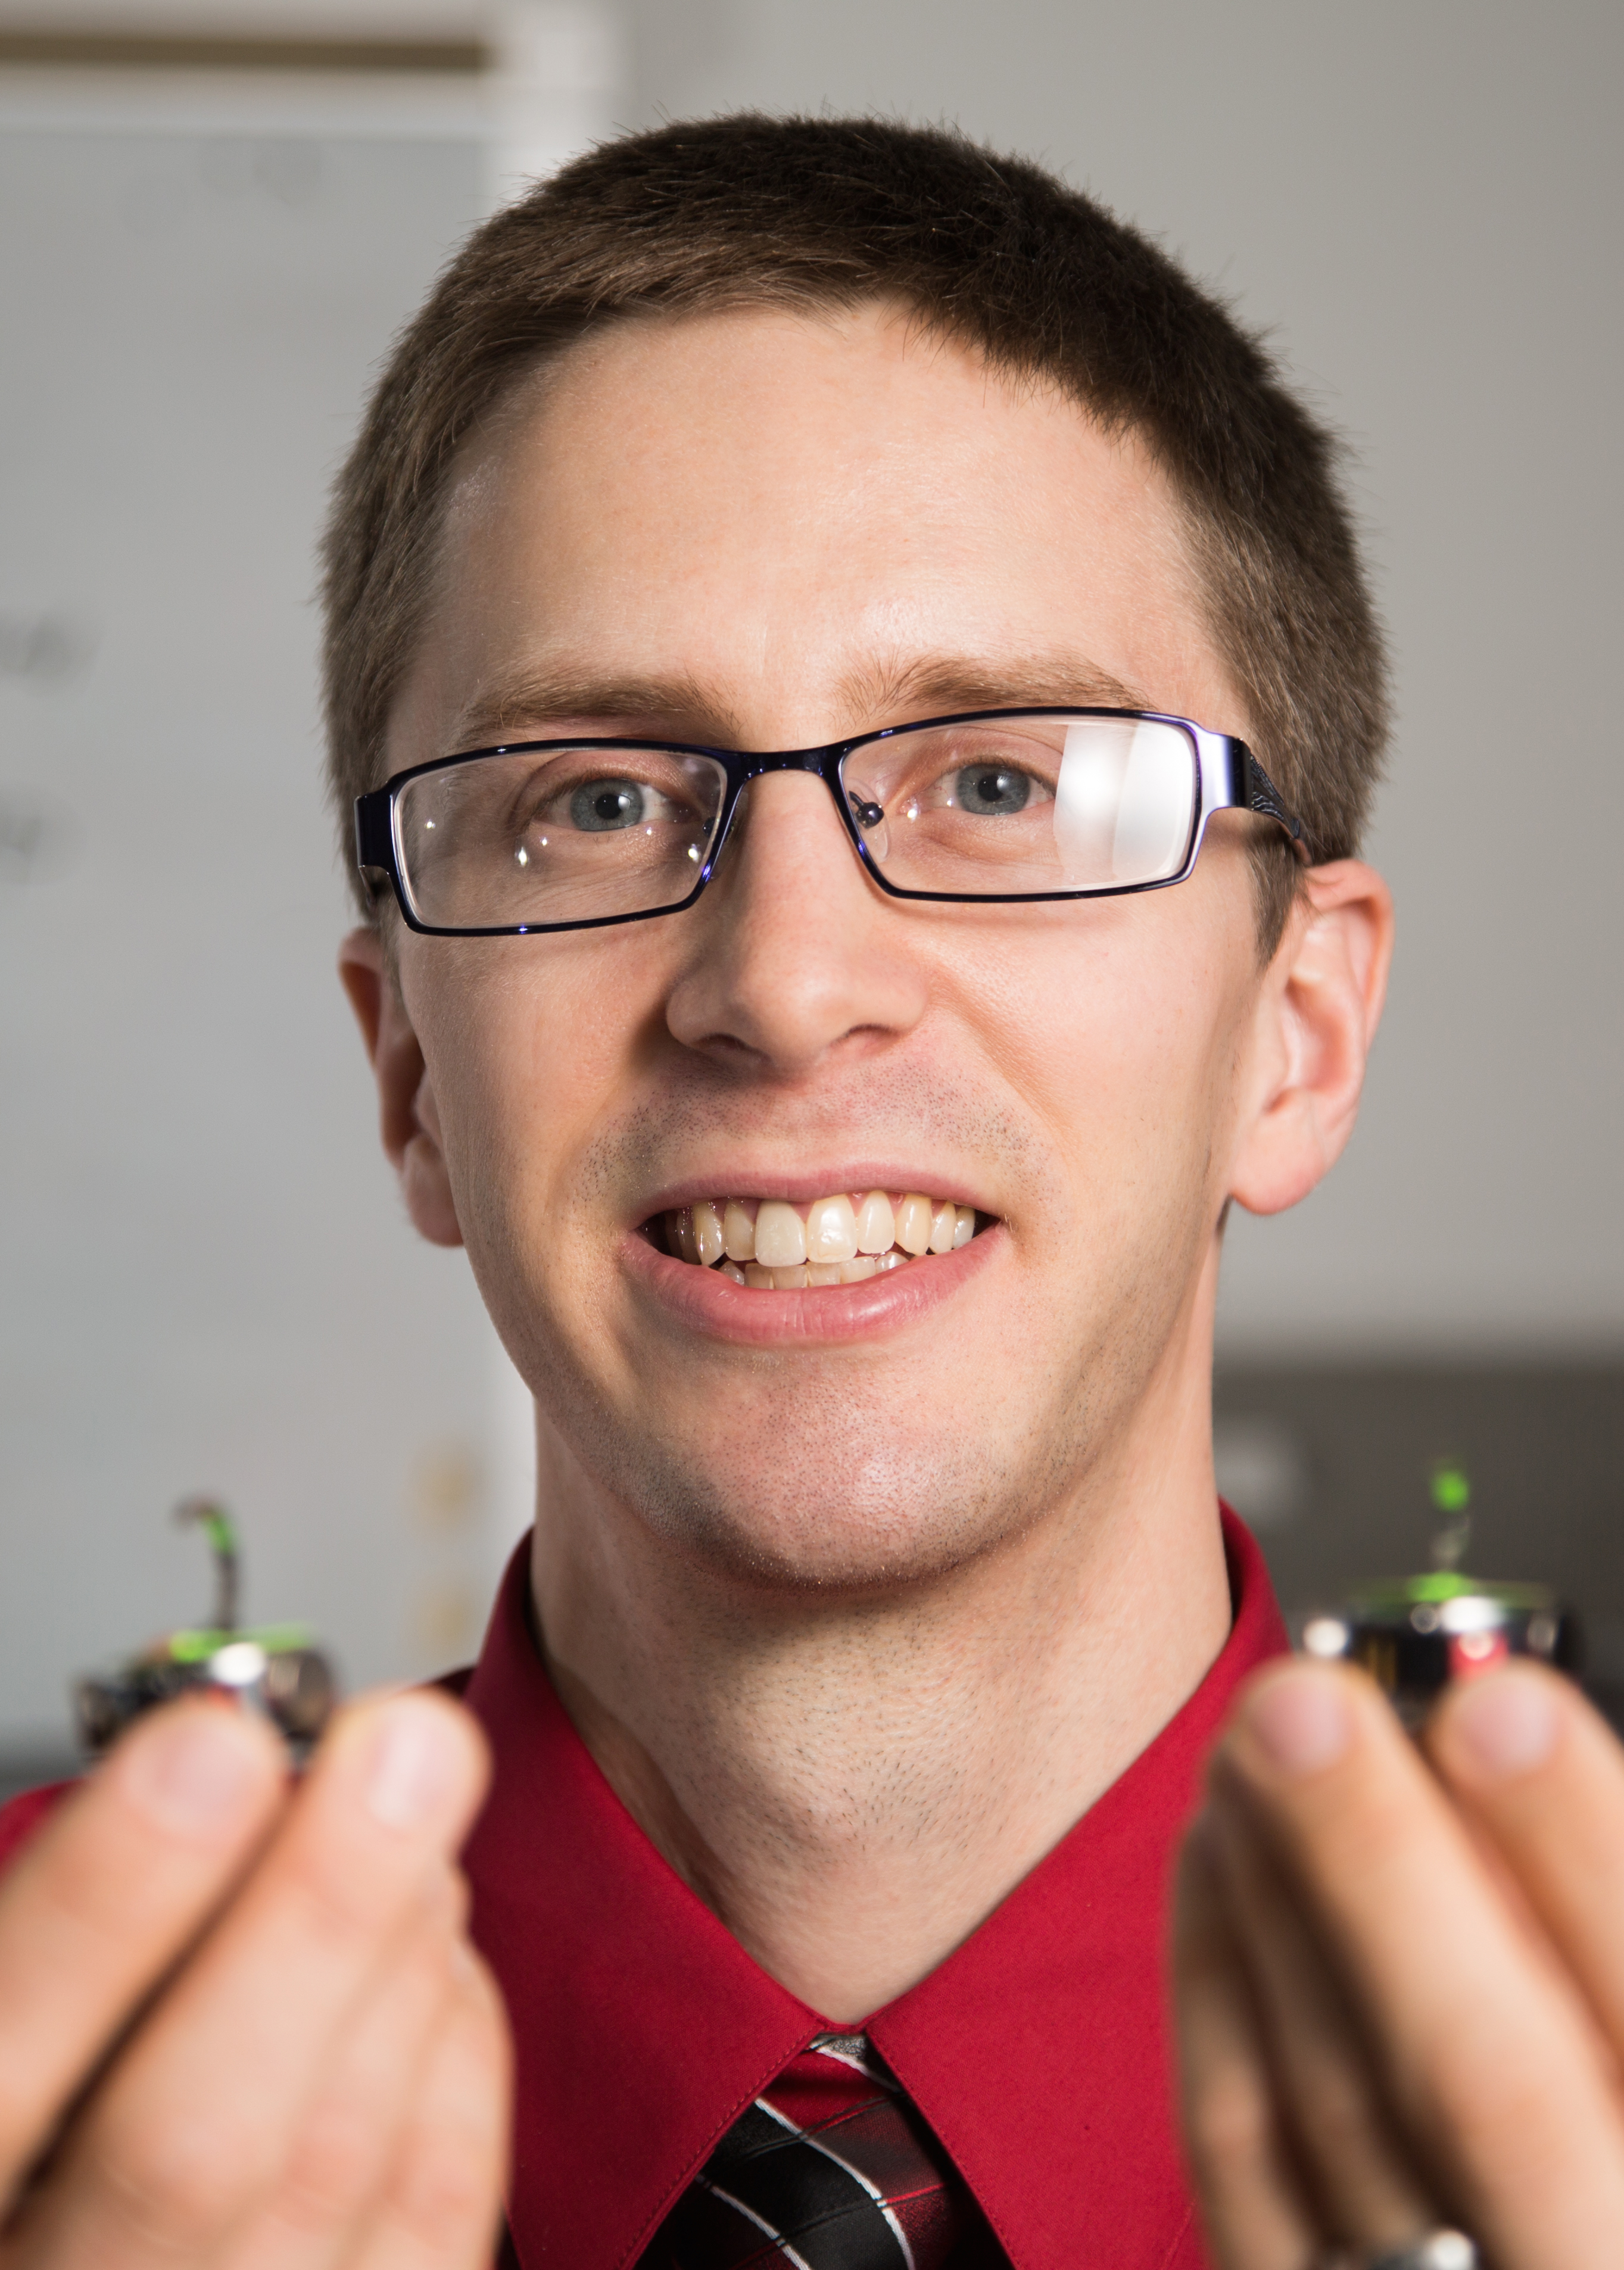
\includegraphics[width=1in,height=1.25in,clip,keepaspectratio]{DrB.jpg}}]{Aaron T. Becker}(S`06-M`12-SM`17) received M.S. and PhD degrees in electrical and computer engineering from the University of Illinois at Urbana-Champaign, in 2008 and 2012. He was a post doctoral research scholar at the Multi-Robot Systems Lab at Rice University and a post doctoral research fellow at Boston Children's Hospital, Harvard Medical School, before joining the Electrical and Computer Engineering Department at the University of Houston as an Assistant Professor in 2014. He won the best paper at IROS 2013 and received the NSF CAREER award in 2016. He is active in developing control laws and algorithms for robot swarms.

\end{IEEEbiography}


\end{document}
